% oneside + openany: PDF de lliurament sense pàgines en blanc entre capítols.
% (twoside/openright és per llibre enquadernat: cada capítol a pàgina senar.)
\documentclass[12pt,a4paper,oneside,openany]{book}

\pdfminorversion=7
\usepackage[T1]{fontenc}
\usepackage[utf8]{inputenc}
\usepackage{lmodern}
\usepackage{mathptmx}
\usepackage[a4paper,top=3.5cm,bottom=3.5cm,left=3cm,right=3cm]{geometry}
\usepackage[english,catalan]{babel}
\usepackage{csquotes}
\usepackage{setspace}
\onehalfspacing
\usepackage{microtype}
\usepackage{graphicx}
\usepackage{booktabs}
\usepackage{tabularx}
\usepackage{longtable}
\usepackage{multirow}
\usepackage{enumitem}
\usepackage{xcolor}
\usepackage{amsmath,amssymb}
\usepackage{tikz}
\usetikzlibrary{arrows.meta,positioning,fit,calc,shapes.geometric}
\usepackage{listings}
\usepackage{caption}
\usepackage{subcaption}
\usepackage{fancyhdr}
\usepackage{etoolbox}
\usepackage{xurl}
\usepackage[backend=biber,style=apa,sorting=nyt,autolang=hyphen]{biblatex}
\addbibresource{bib/referencias.bib}
\usepackage{hyperref}
\usepackage{pdfpages}
\hypersetup{
  colorlinks=true,
  linkcolor=black,
  citecolor=black,
  urlcolor=blue,
  pdflang={ca},
  pdftitle={Studyraft TFM},
}

\lstset{
  basicstyle=\ttfamily\small,
  breaklines=true,
  frame=single,
  columns=fullflexible,
  keepspaces=true,
  showstringspaces=false,
}

\newcommand{\pendiente}[1]{\textbf{\textcolor{red}{[PENDENT: #1]}}}

\setlength{\headheight}{16pt}
\pagestyle{fancy}
\fancyhf{}
\fancyhead[L]{\nouppercase{\leftmark}}
\fancyfoot[C]{\thepage}
\renewcommand{\headrulewidth}{0.3pt}

\setcounter{tocdepth}{2}
\setcounter{secnumdepth}{3}

\addto\captionscatalan{%
  \renewcommand{\contentsname}{Índex}%
  \renewcommand{\listfigurename}{Índex de figures}%
  \renewcommand{\listtablename}{Índex de taules}%
  \renewcommand{\bibname}{Bibliografia}%
  \renewcommand{\chaptername}{Capítol}%
  \renewcommand{\appendixname}{Annex}%
  \renewcommand{\figurename}{Figura}%
  \renewcommand{\tablename}{Taula}%
}

% Completa aquests camps amb la guia oficial del teu centre.

\newcommand{\tfmTipus}{Treball de Fi de Màster}
\newcommand{\tfmTitulo}{Studyraft: assistent d'estudi basat en generació augmentada per recuperació sobre documents propis}
\newcommand{\tfmTitle}{Studyraft: a retrieval-augmented study assistant over personal PDF materials}
\newcommand{\tfmAutor}{Hao Yang}
\newcommand{\tfmTutor}{Jordi Planes Cid}
\newcommand{\tfmCotutor}{} % deixa-ho buit si no hi ha codirector
\newcommand{\tfmUniversidad}{Universitat de Lleida}
\newcommand{\tfmCentro}{Escola Politècnica Superior}
\newcommand{\tfmDepartament}{} % opcional; buit = no es mostra
\newcommand{\tfmMaster}{Màster universitari en Enginyeria Informàtica}
\newcommand{\tfmCurso}{2025/2026}
\newcommand{\tfmConvocatoria}{setembre 2026}
\newcommand{\tfmLloc}{Lleida}
\newcommand{\tfmData}{setembre de 2026}
\newcommand{\tfmKeywordsCA}{RAG, recuperació híbrida, pgvector, arquitectura hexagonal, repetició espaiada, FastAPI, Next.js, RLS}
\newcommand{\tfmKeywordsEN}{RAG, hybrid retrieval, pgvector, hexagonal architecture, spaced repetition, FastAPI, Next.js}


\begin{document}

\hypersetup{pageanchor=false}

\includepdf[pages=-,pagecommand={\thispagestyle{empty}}]{front/portada-oficial.pdf}
\hypersetup{pageanchor=true}

\frontmatter
\chapter*{Resum}
\addcontentsline{toc}{chapter}{Resum}

Aquest treball presenta \emph{Studyraft}, un assistent d'estudi que converteix els PDF propis en un cicle tancat: assignatures, ingestió asíncrona, xat amb cites al fragment d'origen, biblioteca de flashcards i qüestionaris, i repàs amb repetició espaiada (SM-2).

El mètode és un sistema d'enginyeria: arquitectura hexagonal (FastAPI i Next.js, dades a Supabase amb \texttt{pgvector} i RLS), recuperació híbrida (densa, lèxica i fusió RRF), sinopsi de document activa per defecte, i SM-2 al domini. El rerank amb LLM i una passada agentic existeixen com a flags, apagats per defecte.

A data d'1 de setembre de 2026, el backend té 63 tests unitaris verds (\texttt{ruff} i \texttt{mypy} nets); el frontend, 4 tests Vitest i 2 smokes Playwright. Sobre 114 chunks, el retrieval híbrid té p50 de 369\,ms (8 consultes factuals, $k=10$ en aquell run); amb rerank LLM, 1\,608\,ms. L'avaluació mesura programari, latència i un recorregut qualitatiu del cicle; no tanca fidelitat (groundedness).

\paragraph{Paraules clau.}
\tfmKeywordsCA

\tableofcontents
\listoffigures
\listoftables
\chapter*{Llista d'acrònims}
\addcontentsline{toc}{chapter}{Llista d'acrònims}

\begin{description}[style=nextline,leftmargin=3.2cm,labelwidth=3cm]
  \item[ABC] Abstract Base Class (interfície Python dels ports)
  \item[API] Application Programming Interface
  \item[BM25] Best Matching 25 (rànquing lèxic)
  \item[CI] Integració contínua
  \item[CRUD] Create, Read, Update, Delete
  \item[FTS] Full-Text Search
  \item[FSRS] Free Spaced Repetition Scheduler
  \item[GDPR] Reglament general de protecció de dades
  \item[ITS] Intelligent Tutoring System
  \item[JWT] JSON Web Token
  \item[LLM] Large Language Model
  \item[MoSCoW] Must / Should / Could / Won't (priorització de requisits)
  \item[p50] Percentil 50 (mediana) d'una mostra de latències
  \item[RAG] Retrieval-Augmented Generation
  \item[RLS] Row Level Security
  \item[RRF] Reciprocal Rank Fusion
  \item[RSC] React Server Components
  \item[SM-2] SuperMemo 2 (repetició espaiada)
  \item[SRS] Spaced Repetition System
  \item[SSE] Server-Sent Events
  \item[TFM] Treball de Fi de Màster
\end{description}


\mainmatter
\chapter{Introducció i objectius}
\label{cap:intro}

\section{Motivació}

Estudiar a partir d'apunts i llibres en PDF és el cas d'ús quotidià d'un estudiant d'enginyeria, però les eines genèriques de \emph{xat amb documents} no cobreixen el cicle complet d'aprenentatge. Un model de llenguatge sense recuperació tendeix a al·lucinar; un cercador semàntic sense cites no es pot auditar; un generador de flashcards sense espaiat temporal no consolida la memòria. L'estudiant necessita un sistema que (i)~parteixi dels \emph{seus} documents, (ii)~respongui amb evidència localitzable i (iii)~converteixi aquest context en pràctica (targetes, test, repàs) i en una \emph{biblioteca} de materials que es pugui editar i reutilitzar.

Productes comercials (Quizlet, Anki, NotebookLM, ChatGPT amb fitxers) cobreixen fragments d'aquest cicle, però no combinen de manera oberta: multiassignatura, ingestió asíncrona auditable, recuperació híbrida, cites clicables, generació d'estudi, repetició espaiada i persistència de conjunts, amb una arquitectura mantenible i avaluable en un TFM.

\section{Problema}

Donat un conjunt de PDF privats d'un usuari, es vol:

\begin{enumerate}
  \item Extreure, trossejar i representar el contingut de manera recuperable.
  \item Respondre preguntes \emph{ancorades} a fragments, amb nom de fitxer i interval de pàgines.
  \item Generar materials de pràctica (flashcards i qüestionaris) a partir del mateix índex, i conservar-los com a conjunts amb títol.
  \item Programar el repàs amb un algoritme de repetició espaiada traçable.
\end{enumerate}

Cal un \emph{sistema}: límits de confiança, aïllament per usuari (RLS), cues d'ingestió, observabilitat d'etapes i una interfície que no barregi cinc tasques a la mateixa pantalla. Invocar un model de llenguatge n'és només una peça.

\section{Contribucions}

Aquest TFM aporta, sobre el producte \emph{Studyraft}:

\begin{itemize}
  \item Una reconstrucció completa amb \textbf{arquitectura hexagonal} (domini sense I/O, ports, adaptadors, entrypoints) després d'un llegat amb LangChain.
  \item Un \textbf{pipeline d'ingestió per etapes} (\texttt{download} $\rightarrow$ \texttt{parse} $\rightarrow$ \texttt{chunk} $\rightarrow$ \texttt{embed} $\rightarrow$ \texttt{store} $\rightarrow$ \texttt{synopsis}), relançable i depurable, amb worker asíncron dins FastAPI.
  \item \textbf{RAG híbrid} (dens + lèxic + Reciprocal Rank Fusion), amb rerank LLM opcional, índex jeràrquic de sinopsi, classificació d'intent (resum / capítol / factual) i una passada agentic opcional.
  \item Un \textbf{cicle d'estudi} en Next.js~16 i React~19: xat amb streaming i cites, biblioteca de flashcards i qüestionaris (generats, manuals o importats), editors, pistes a la pràctica i planner SM-2.
  \item Un \textbf{protocol de qualitat}: tests unitaris, tipus (mypy/tsc), lint, smoke E2E i un CLI de benchmark de recuperació.
\end{itemize}

\section{Objectius}

\paragraph{Objectiu general.}
Dissenyar, implementar i avaluar un assistent d'estudi RAG sobre documents propis, amb arquitectura desacoblada i un cicle de pràctica verificable.

\paragraph{Objectius específics.}
\begin{enumerate}[label=O\arabic*.]
  \item Formalitzar requisits funcionals i no funcionals del cicle assignatura--document--xat--pràctica.
  \item Implementar ingestió asíncrona amb persistència d'estat per etapa.
  \item Implementar recuperació híbrida amb cites enriquides (fitxer, pàgines, fragment) i política lecture-focused.
  \item Implementar generació i biblioteca de flashcards/qüestionaris, i repàs SM-2.
  \item Exposar una API autenticada (JWT de Supabase) i una UI coherent amb el sistema de disseny Studyraft.
  \item Definir i executar un protocol d'avaluació (tests + latència de retrieval + limitacions).
\end{enumerate}

O1--O5 són objectius d'\emph{implementació}: es consideren coberts si existeix ruta API, UI o CLI, i almenys un test (unitari o d'integració). O6 és d'\emph{avaluació}: no es tanca amb un pytest. Queda \emph{parcial} amb el protocol del capítol~\ref{cap:resultados} (qualitat de programari, latència de retrieval, recorregut qualitatiu del cicle a la UI). Resta obert: fidelitat (groundedness), contrast només dens, durada d'ingestió, latència extrem a extrem del xat, i un estudi amb alumnes.

\section{Abast i no-abast}

Dins d'abast: PDF de text extraïble, un usuari autenticat, una assignatura com a unitat d'aïllament, OpenAI o Gemini com a proveïdors LLM, Supabase allotjat, desplegament local amb Docker Compose. L'\textbf{idioma de la interfície} del producte és el castellà de tu; l'\textbf{idioma d'aquesta memòria} és el català.

Fora d'abast (i es reprenen al capítol~\ref{cap:conclusiones}): OCR de PDF escanejats, visor PDF a pàgina completa, agent RAG multi-eina, desplegament multiregió de producció, exportació Anki \texttt{.apkg} i un estudi d'usuaris amb $n$ estadísticament significatiu.

\section{Àmbit temporal i dedicació}
\label{sec:ambit-temporal}

El calendari es reconstrueix a partir de Git: el primer commit és del 9 de desembre de 2025 i l'últim de producte, del 28 d'agost de 2026; la memòria es tanca l'1 de setembre. El període no és un sprint continu: hi ha pauses (sobretot març i juny de 2026) i un canvi de baseline el 8 de juliol, quan s'arxiva el prototip LangChain i es reescriu el sistema en hexagonal. Els 19 commits són entregues de gran volum, no un registre diari. Les hores de la taula~\ref{tab:ambit-temporal} són una estimació de dedicació (disseny, implementació, depuració i redacció), calibrada amb el volum de canvi i amb el mínim acadèmic de \textbf{360 hores}. El total estimat és de \textbf{390 hores}. Producte i memòria se solapen a l'agost, com és habitual en un TFM.

\begin{table}[htbp]
\centering
\caption{Planificació temporal (històric de Git, 2025--2026) i dedicació estimada.}
\label{tab:ambit-temporal}
\small
\begin{tabularx}{\textwidth}{@{}>{\raggedright\arraybackslash}p{3.15cm} >{\raggedright\arraybackslash}p{2.55cm} c r X@{}}
\toprule
Fase & Període & Setm. & Hores & Tasques resumides \\
\midrule
Recerca i prototip RAG
  & 09/12/2025 -- 05/01/2026
  & 4 & 35
  & Commit inicial; pipeline FastAPI; \texttt{backend\_v2} i RAG agentic. \\
Prototip UI i pràctica
  & 03/02/2026 -- 27/02/2026
  & 4 & 35
  & Kit d'UI; pàgines de quiz i estudi amb històric. \\
LLM, Supabase i API
  & 24/04/2026 -- 13/05/2026
  & 3 & 45
  & Proveïdors LLM/embeddings; repositori; JWT; client API i navegació. \\
Reescriptura hexagonal
  & 08/07/2026 -- 29/07/2026
  & 3 & 75
  & Arxiu del llegat; esquema SQL/RLS; ports i adaptadors; API i tests. \\
Frontend Studyraft
  & 29/07/2026 -- 12/08/2026
  & 2 & 65
  & Auth SSR, assignatures, documents, xat, pràctica i CI de frontend. \\
Qualitat, planner i Docker
  & 12/08/2026 -- 23/08/2026
  & 2 & 45
  & Quality gates; streaming i rerank; RAG lecture-focused; Compose. \\
Biblioteca d'estudi
  & 23/08/2026 -- 28/08/2026
  & 1 & 20
  & Conjunts de flashcards/quiz, CRUD, recència, pistes, import/export. \\
Redacció de la memòria
  & 01/08/2026 -- 01/09/2026
  & 4 & 50
  & Cos \LaTeX{}, estat de l'art, requisits, arquitectura i annexos. \\
Seguiment i revisions
  & 09/12/2025 -- 31/08/2026
  & --- & 20
  & Reunions amb el director, ajust d'abast i revisions parcials. \\
\midrule
\multicolumn{3}{@{}l}{\textbf{Total}} & \textbf{390} & \\
\bottomrule
\end{tabularx}
\end{table}

\begin{figure}[htbp]
\centering
% Gantt simplificat (des. 2025 -- ago. 2026). Les pauses (març, juny) es veuen com a buits.
\begin{tikzpicture}[
  font=\scriptsize,
  x=0.68cm, y=0.44cm,
  bar/.style={fill=black!18, draw=black!50, thin},
]
\foreach \x/\m in {0/des.,1/gen.,2/feb.,3/mar.,4/abr.,5/mai.,6/jun.,7/jul.,8/ago.} {
  \node[anchor=south] at (3.3+\x+0.4, 8.45) {\m};
  \draw[black!18] (3.3+\x, 0.1) -- (3.3+\x, 8.25);
}
\draw[black!45] (3.3,0.1) -- (12.3,0.1);
\providecommand{\tfmganttbar}[4]{%
  \node[anchor=east, align=right] at (3.15,#1) {#4};
  \fill[bar] (3.3+#2,#1-0.32) rectangle (3.3+#3,#1+0.32);
}
\tfmganttbar{7.5}{0.2}{1.1}{Prototip RAG}
\tfmganttbar{6.5}{2.05}{2.9}{UI / pràctica}
\tfmganttbar{5.5}{4.7}{5.45}{LLM i API}
\tfmganttbar{4.5}{7.15}{7.95}{Hexàgon}
\tfmganttbar{3.5}{7.85}{8.4}{Frontend}
\tfmganttbar{2.5}{8.3}{8.75}{Qualitat}
\tfmganttbar{1.5}{8.65}{8.95}{Biblioteca}
\tfmganttbar{0.5}{7.95}{9.0}{Memòria}
\end{tikzpicture}

\caption{Diagrama de Gantt simplificat (desembre 2025 -- agost 2026). Els buits (sobretot març i juny) són pauses reals de Git, no sprints continus.}
\label{fig:gantt}
\end{figure}

A 25\,€/hora (tarifa acadèmica habitual en TFM, no de mercat), el cost estimat de la dedicació és de \textbf{9.750\,€}. El projecte és de recerca i aprenentatge, no d'explotació comercial: un pas a producció (allotjament, quotes d'API, manteniment) quedaria fora d'aquest pressupost. El cost variable d'API (embeddings i xat) és a la secció~\ref{sec:cost-api}. El detall de fases d'enginyeria es reprèn al capítol~\ref{cap:gestion}.

\section{Estructura de la memòria}

El capítol~\ref{cap:arte} situa el treball a la literatura. El~\ref{cap:requisitos} fixa requisits. Els capítols~\ref{cap:arquitectura} i~\ref{cap:desarrollo} descriuen disseny i implementació de l'estat actual del repositori. El~\ref{cap:resultados} defineix l'avaluació. El~\ref{cap:gestion} cobreix planificació, riscos i ètica. El~\ref{cap:conclusiones} tanca amb conclusions i línies futures.

\chapter{Estat de l'art}
\label{cap:arte}

El fil d'aquest capítol és el mateix que el del problema (capítol~\ref{cap:intro}): un estudiant amb PDF propis no necessita un model de llenguatge aïllat, ni una app de flashcards aïllada, ni un cercador aïllat. Necessita un \textbf{cicle} amb quatre baules encadenades (figura~\ref{fig:cicle}):

\begin{enumerate}
  \item \textbf{Indexar} documents privats de manera recuperable (trossejar i representar).
  \item \textbf{Recuperar} el fragment adequat (i poder-lo citar).
  \item \textbf{Generar} una resposta o un material de pràctica \emph{ancorat} a aquest fragment.
  \item \textbf{Programar el repàs} perquè el que s'ha practicat no es perdi.
\end{enumerate}

\begin{figure}[htbp]
\centering
\begin{tikzpicture}[
  font=\small,
  box/.style={draw, rounded corners=2pt, align=center, inner sep=6pt,
    minimum width=2.55cm, minimum height=1.35cm},
  arr/.style={-{Latex[length=2.2mm]}, thick}
]
\node[box] (a) {1. Indexar\\PDF privat};
\node[box, right=0.45cm of a] (b) {2. Recuperar\\amb evidència};
\node[box, right=0.45cm of b] (c) {3. Generar\\ancorat};
\node[box, right=0.45cm of c] (d) {4. Repassar\\SM-2};
\draw[arr] (a) -- (b);
\draw[arr] (b) -- (c);
\draw[arr] (c) -- (d);
\end{tikzpicture}

\caption{Les quatre baules del cicle d'estudi que articulen aquest capítol.}
\label{fig:cicle}
\end{figure}

La literatura i el mercat cobreixen cada baula per separat, sovint amb molta profunditat. El que gairebé no existeix ---i el que aquest TFM reivindica--- és tancar el cicle de forma \emph{oberta, limitada i avaluable}, com un sistema d'enginyeria i no com un notebook. El detall de FastAPI, Next.js o Supabase no pertany aquí: és disseny (capítols~\ref{cap:arquitectura} i~\ref{cap:desarrollo}).

\section{De l'LLM nu al RAG}

Un LLM sense evidència externa respon amb el que ha memoritzat a l'entrenament. Això falla en apunts d'una assignatura concreta: el model no ha vist \emph{aquest} PDF, i si improvisa no hi ha manera d'auditar-lo. Lewis et al. \parencite{lewis2020rag} van formular la generació augmentada per recuperació (RAG) com la combinació d'un retriever i un generador condicionat als documents recuperats. La promesa és reduir al·lucinacions: la resposta ha de dependre d'un context extern, no només dels paràmetres del model.

A la pràctica, la qualitat depèn més de \emph{què} es recupera que de la mida de l'LLM \parencite{gao2024retrieval}. Per a aquest treball, això talla una via: no cal un model fronterer; cal un retriever honest, cites localitzables i un prompt que prohibeixi inventar fora del context. RAG cobreix, doncs, les baules~2 i~3 \emph{quan la tasca és preguntar}. Encara no diu com s'indexa un PDF de classe, ni com es practica després.

\section{Indexar: trossejar abans de recuperar}

La baula~1 no és ``pujar un fitxer a un xat''. És decidir \emph{quin} fragment entrarà a l'índex. Un PDF de 60 pàgines no cap sencer al retriever; es parteix en \emph{chunks}. Si el tall cau a mitja definició, ni BM25 ni l'embedding recuperen una unitat útil. Si els chunks són massa llargs, el model pot ``perdre'' el fet rellevant al mig del context \parencite{liu2024lost}. Barnett et al. \parencite{barnett2024seven} resumeixen set punts de fallada d'un RAG en producció; els primers són d'indexació (contingut absent o mal trossejat), no de l'LLM.

La taula~\ref{tab:chunking} contraposa estratègies habituals. Studyraft no inventa un algorisme nou: aplica una cascada (capçaleres $\rightarrow$ paràgrafs $\rightarrow$ oracions $\rightarrow$ tall dur) amb màxim 1200 caràcters i solapament 150 (capítol~\ref{cap:desarrollo}). El solapament redueix frases partides; duplica uns quants tokens d'embedding, un cost negligible (secció~\ref{sec:cost-api}).

\begin{table}[htbp]
\centering
\caption{Estratègies de trossejat (chunking) i el risc que arrosseguen.}
\label{tab:chunking}
\small
\begin{tabularx}{\textwidth}{lXX}
\toprule
Estratègia & Idea & Risc típic \\
\midrule
Finestra fixa & $N$ caràcters, independent de l'estructura. & Talla definicions i títols. \\
Finestra + solapament & El final d'un chunk es repeteix al següent. & Recupera ponts; duplica tokens. \\
Per capçaleres & Un chunk $\approx$ una secció del PDF. & Molts apunts no tenen títols detectables. \\
Studyraft (aquest TFM) & Cascada semàntica, $N{=}1200$, solapament 150, pàgines al metadada. & Sense OCR; un escaneig no genera chunks. \\
\bottomrule
\end{tabularx}
\end{table}

\section{Recuperar sobre apunts reals}

La baula~2 no és un únic algoritme. La cerca densa (embeddings + índex vectorial) captura paràfrasis: ``què és el potencial d'acció?'' \parencite{karpukhin2020dpr}. La cerca lèxica (BM25 / FTS) captura identificadors, fórmules i termes rars: ``què diu de $Na^+$ a la pàgina 12?'' \parencite{robertson2009probabilistic}. Un corpus d'apunts d'enginyeria barreja totes dues consultes; quedar-se només amb embeddings deixa escapar el que l'estudiant copia literalment del PDF.

Quan no es vol entrenar un model de fusió, Reciprocal Rank Fusion és un component estàndard per combinar llistes \parencite{cormack2009rrf}. Un rerank amb LLM millora sovint el top-$k$, a costa de latència i tokens: és un compromís de producte, no un requisit teòric (al capítol~\ref{cap:resultados} el p50 passa de 369\,ms a 1\,608\,ms). El fil és clar: RAG exigeix evidència; sobre apunts, l'evidència s'obté millor amb senyal densa \emph{i} lèxica, fusionades, i cites que mostrin fitxer i pàgina.

\begin{table}[htbp]
\centering
\caption{Senyals de recuperació sobre apunts (no és un ranking experimental).}
\label{tab:senyals}
\small
\begin{tabularx}{\textwidth}{lXX}
\toprule
Senyal & Què encerta & Què falla sol \\
\midrule
Dens (embedding) & Paràfrasi, sinònims, pregunta ``en les meves paraules''. & Sigles, fórmules, números de capítol. \\
Lèxic (BM25/FTS) & Termes rars i còpia literal del PDF. & Reformulacions sense paraules en comú. \\
Híbrid + RRF & Uneix les dues llistes sense un model de fusió entrenat. & Encara pot situar un chunk irrellevant al top-$k$. \\
+ rerank LLM & Reordena llegint pregunta i fragment. & Latència i cost; no substitueix un bon índex. \\
\bottomrule
\end{tabularx}
\end{table}

\section{Fidelitat: que la resposta estigui al chunk}

Recuperar un chunk no garanteix que la frase generada en depengui. La \emph{groundedness} (o fidelitat) és la propietat que cada afirmació de la resposta estigui suportada pel context recuperat. Protocols com RAGAS operacionalitzen això amb mètriques automàtiques (p.~ex. \emph{faithfulness}) \parencite{es2024ragas}. Gao et al. \parencite{gao2024retrieval} insisteixen que avaluar només la fluïdesa de l'LLM amaga al·lucinacions ben redactades.

Aquest TFM \textbf{no tanca} aquesta mètrica: exigiria anotació o un jutge LLM amb protocol (capítol~\ref{cap:resultados}). El que sí fa el sistema és \emph{reduir la superfície} d'invenció: prompt que prohibeix sortir del context, cites amb snippet, i (opcional) filtre lecture-focused. Això és enginyeria de producte, no una prova de fidelitat.

\section{Quan una sola passada no basta}

Fins aquí s'assumeix una pregunta puntual i uns quants chunks. Les preguntes d'estudi sovint són àmplies (``de què va aquest tema?'') o de capítol. Un índex jeràrquic (sinopsi de document $\rightarrow$ fragments) ajuda a no quedar-se només amb el fragment la frase del qual s'assembla a la pregunta. Els enfocaments agentic ---reescriure la consulta i tornar a recuperar, o crítiques com Self-RAG--- milloren la cobertura \parencite{asai2024selfrag}, però converteixen un \texttt{retrieve} en un bucle: cost, no-determinisme i més superfície d'error.

Per a un TFM, aquestes extensions existeixen, tenen sentit en un subconjunt de preguntes i s'han d'acotar (flags, una sola reescriptura). El cicle d'estudi no s'atura en recuperar millor: encara falta convertir l'evidència en pràctica.

\section{Més enllà del xat: pràctica i calendari}

Un xat citat tanca una sessió de dubtes; no consolida memòria. La baula~3, en un assistent d'estudi, també és \emph{generar} flashcards i qüestionaris a partir del mateix índex, i conservar-los com a conjunts editables. La baula~4 és programar el repàs.

SM-2 \parencite{wozniak1990supermemo} continua sent l'algoritme de referència pedagògic (Anki el va popularitzar). No és el model de memòria més recent: Half-Life Regression estima la vida mitjana d'un ítem a partir de l'historial de pràctica \parencite{settles2016hlr}; FSRS ajusta intervals amb més paràmetres a partir dels logs de ressenya \parencite{ye2024fsrs}. En un TFM d'enginyeria, la traçabilitat ---poder explicar per què una carta surt avui amb una fórmula tancada al domini--- pesa més que un petit guany de calendari. RAG dóna el context; SM-2 evita que el context sigui només una conversa efímera.

\section{Sistemes acadèmics (no només productes)}

La taula~\ref{tab:relacionados} compara apps de mercat. El tribunal també pregunta què hi ha a la \emph{literatura} de sistemes, no al catàleg comercial. Dues famílies són útils com a contrast, no com a rivals a ``guanyar'':

\begin{itemize}
  \item \textbf{RAG sobre documents amb cites.} PaperQA recupera fragments de papers científics i obliga a citar-los en la resposta \parencite{lala2023paperqa}. Comparteix amb Studyraft el problema de la baula~2+3 (evidència localitzable). No tanca flashcards ni SRS sobre els apunts de l'estudiant.
  \item \textbf{Tutoria intel·ligent (ITS).} Sistemes com AutoTutor i la revisió de VanLehn mostren que un tutor amb \emph{model de l'alumne} pot acostar-se, en alguns dominis, a un tutor humà \parencite{graesser2005autotutor,vanlehn2011tutoring}. Studyraft no modela l'estudiant més enllà de SM-2: no diagnostica concepcions errònies ni adapta un currículum.
\end{itemize}

\begin{table}[htbp]
\centering
\caption{Contrast acadèmic: cada sistema tanca un tros del cicle.}
\label{tab:academics}
\small
\begin{tabularx}{\textwidth}{lXX}
\toprule
Sistema & Què cobreix & Què no és aquest TFM \\
\midrule
PaperQA & RAG + cites sobre papers. & No és un cicle d'estudi (cards/SRS) sobre PDF de classe. \\
ITS (AutoTutor / VanLehn) & Tutoria amb model de l'alumne. & No indexa els apunts privats de l'estudiant. \\
HLR / Duolingo & SRS a escala amb model estadístic. & No recupera fragments d'un PDF propi. \\
Studyraft & Quatre baules, MVP avaluable. & Sense model cognitiu ric ni mètrica de fidelitat. \\
\bottomrule
\end{tabularx}
\end{table}

\section{Per què això ha de ser un sistema, no un notebook}

Totes les baules anteriors es poden demostrar en un colab: un PDF, uns embeddings, un prompt. Un TFM d'enginyeria informàtica ha d'argumentar \emph{modularitat i aïllament}: usuaris que no es veuen les dades, cues d'ingestió, substitució de proveïdor LLM, tests amb dobles. L'arquitectura hexagonal (ports i adaptadors) \parencite{cockburn2005hexagonal} és el marc clàssic per a això: el cas d'ús no coneix ni HTTP ni el client de base de dades.

Aquesta secció no compara frameworks de moda. Justifica una exigència del tribunal: el cicle d'estudi ha de ser llegible al codi i limitable (sense OCR, sense agent general, amb RLS). Les tecnologies concretes es trien al capítol~\ref{cap:arquitectura}.

\section{El mercat: cada producte tanca un tros del cicle}

Els productes comercials confirmen el diagnòstic. Anki i Quizlet excel·leixen a la pràctica i, en graus diversos, al calendari, però no parteixen dels PDF de l'estudiant amb cites. NotebookLM i el xat amb fitxers indexen documents i citen, però no tanquen flashcards, quiz persistents i SRS com a cicle d'estudi. La taula~\ref{tab:relacionados} és una \textbf{cobertura declarada} (agost de 2026, ús de les interfícies públiques conegudes), \emph{no} un ranking ni una avaluació empírica: Studyraft no «guanya»; ocupa la casella d'integració que aquest TFM construeix.

\begin{table}[htbp]
\centering
\caption{Cobertura declarada del cicle d'estudi (agost 2026). Pràctica = flashcards i qüestionaris. No és un ranking de qualitat.}
\label{tab:relacionados}
\small
\begin{tabular}{lcccc}
\toprule
Sistema & PDF propis & Cites & Pràctica & SRS \\
\midrule
Anki & no natiu & no & sí & sí \\
Quizlet & limitat & no & sí & limitat \\
NotebookLM & sí & sí & limitat & no \\
ChatGPT + fitxers & sí & variable & no & no \\
Studyraft & sí & sí & sí & sí (SM-2) \\
\bottomrule
\end{tabular}
\end{table}

\section{Posicionament}

El forat que ocupa aquest treball no és un nou algoritme de retrieval de primer nivell, ni un nou model de memòria. És la \textbf{integració avaluable} de les quatre baules ---indexar, recuperar amb cites, practicar, repassar--- sobre documents privats, amb una arquitectura que es pugui llegir, provar i limitar. Les seccions anteriors expliquen \emph{per què} cada baula existeix a la literatura; els capítols de disseny i desenvolupament expliquen \emph{com} Studyraft les encadena.

\chapter{Anàlisi i requisits}
\label{cap:requisitos}

\section{Actors i context}

L'actor principal és un \textbf{estudiant autenticat}. El sistema no exposa dades entre usuaris: totes les files de negoci porten \texttt{user\_id} i polítiques RLS a Postgres. Un segon actor tècnic és el \textbf{worker d'ingestió}, que reclama treballs en cua (\texttt{claim\_next\_job}) dins del procés FastAPI. No hi ha rol d'administrador a l'MVP: qui desplega el projecte Supabase té accés de plataforma, fora de la UI.

\section{Cas d'ús principal}

El flux mínim implementat al producte és:

\begin{enumerate}
  \item Registre / login (correu i contrasenya; restabliment via enllaç). El proveïdor d'Auth admet OAuth; aquest MVP no l'exposa a la UI (annex~\ref{anexo:despliegue}).
  \item Crear una assignatura (onboarding si no n'hi ha cap).
  \item Pujar un PDF, seguir l'estat (\emph{en cua} / \emph{processant} / \emph{llest} / error) i, si cal, reindexar.
  \item Preguntar al xat (amb àmbit de documents opcional), llegir la resposta en streaming i obrir cites (nom de PDF + fragment).
  \item Generar flashcards o un qüestionari; conservar-los a la biblioteca; practicar o editar; importar/exportar JSON.
  \item Al planner, puntuar qualitat SM-2 de les targetes vençudes.
  \item Ajustar el perfil (nom visible, flag de RAG agentic).
\end{enumerate}

\begin{figure}[htbp]
\centering
\begin{tikzpicture}[
  font=\small,
  actor/.style={draw, rounded corners=2pt, align=center, inner sep=4pt, minimum width=2.2cm},
  uc/.style={draw, ellipse, align=center, inner sep=3pt, minimum width=3.3cm, minimum height=0.85cm}
]
\node[actor] (est) {Estudiant\\autenticat};
\node[uc, right=1.6cm of est] (asig) {Gestionar assignatures};
\node[uc, below=0.28cm of asig] (pdf) {Pujar i indexar PDF};
\node[uc, below=0.28cm of pdf] (xat) {Preguntar amb cites};
\node[uc, below=0.28cm of xat] (gen) {Generar i editar pràctica};
\node[uc, below=0.28cm of gen] (srs) {Repassar (SM-2)};
\node[actor, right=1.5cm of gen] (wrk) {Worker\\d'ingestió};
\draw (est.east) -- (asig.west);
\draw (est.east) -- (pdf.west);
\draw (est.east) -- (xat.west);
\draw (est.east) -- (gen.west);
\draw (est.east) -- (srs.west);
\draw (wrk.west) -- (pdf.east);
\end{tikzpicture}

\caption{Casos d'ús de l'MVP. L'estudiant inicia el cicle; el worker completa la indexació.}
\label{fig:usecases}
\end{figure}

\paragraph{Pre- i postcondició (cas d'ús de xat).}
Pre: hi ha almenys un document en estat llest a l'assignatura. Flux: l'estudiant envia una pregunta; el sistema classifica, recupera, genera amb cites i (si cal) desa el fil. Post: la UI mostra la resposta i les cites; no s'ha cridat l'LLM amb la clau al navegador.

\paragraph{Escenaris d'error.}
PDF sense text extraïble: l'etapa \texttt{parse} falla i l'estat del document és error (no s'inventa OCR). Job d'ingestió fallit: l'usuari pot reindexar (RF-04). JWT caducat o invàlid: l'API respon 401. Assignatura o document d'un altre usuari: 404 (no es filtra l'existència aliena). Context insuficient al xat: el prompt obliga a dir-ho, no a inventar.

\section{Requisits funcionals}

La taula~\ref{tab:rf} recull els requisits coberts per l'API i la UI actuals (extracte; el contracte complet és a l'annex~\ref{anexo:esquema}). La prioritat és MoSCoW: \emph{Must} per a l'MVP del cicle, \emph{Should} per a preferències, \emph{Could} per a depuració.

\begin{table}[htbp]
\centering
\caption{Requisits funcionals implementats i prioritat.}
\label{tab:rf}
\small
\begin{tabularx}{\textwidth}{lcX}
\toprule
Id & Prior. & Requisit \\
\midrule
RF-01 & Must & L'usuari gestiona assignatures (CRUD). \\
RF-02 & Must & L'usuari puja PDF associats a una assignatura (límit 25\,MB). \\
RF-03 & Must & El sistema indexa el PDF de manera asíncrona i n'informa l'estat. \\
RF-04 & Must & L'usuari pot reintentar una ingestió fallida (reindex). \\
RF-05 & Must & El xat respon fent servir només context recuperat, amb cites (fitxer, pàgines, snippet). \\
RF-06 & Must & El xat suporta streaming SSE i historial de fils per assignatura. \\
RF-07 & Must & Es generen flashcards i qüestionaris a partir de l'índex (lecture-focused). \\
RF-08 & Must & La biblioteca persisteix conjunts amb títol, origen, recompte i data d'actualització. \\
RF-09 & Must & Es poden crear, editar, esborrar, importar i exportar cartes i preguntes. \\
RF-10 & Must & El planner llista targetes vençudes i registra ressenyes SM-2. \\
RF-11 & Should & El perfil persisteix preferències de retrieval (p.~ex. agentic). \\
RF-12 & Could & Un mode debug (flag) permet executar rangs de pipeline. \\
\bottomrule
\end{tabularx}
\end{table}

\section{Requisits no funcionals}

\begin{itemize}
  \item \textbf{Seguretat.} Autenticació JWT Supabase (HS256); autorització per \texttt{user\_id} a cada cas d'ús; RLS amb \texttt{(select auth.uid())} al client; el navegador no posseeix claus d'LLM. No hi ha SLA ni pentest en aquest TFM.
  \item \textbf{Mida i recuperació.} Pujada màxima 25\,MB (\texttt{MAX\_UPLOAD\_SIZE\_BYTES}); cerca densa i lèxica amb $k=20$ i context final $k=8$. La latència d'ingestió i de xat \emph{no} es garanteix: depèn d'APIs externes.
  \item \textbf{Mantenibilitat.} Domini sense imports de FastAPI/Supabase/OpenAI; ports ABC; tests amb fakes; factory OpenAI/Gemini.
  \item \textbf{Observabilitat.} Estats de job i \texttt{pipeline\_stage\_runs}; telemetria OpenTelemetry opcional.
  \item \textbf{Qualitat de lliurament.} \texttt{ruff}, \texttt{mypy --strict}, pytest unitari, \texttt{tsc}, Vitest, Playwright smoke, Docker Compose, CI a GitHub Actions.
  \item \textbf{Usabilitat.} Una tasca per pantalla; interfície en castellà de tu; cites amb nom de fitxer; el hover no és l'única via de navegació.
\end{itemize}

\section{Restriccions}

\begin{itemize}
  \item PDF amb text extraïble (PyPDF); no hi ha OCR a l'MVP.
  \item Dependència d'APIs d'embeddings/LLM (cost i latència externs).
  \item Supabase allotjat (l'esquema viu a les migracions SQL del repositori).
  \item El flag \texttt{ENABLE\_RATE\_LIMIT} existeix (defecte \texttt{true} a la configuració), però \textbf{no hi ha middleware de quota implementat}. És deute conegut: el flag no s'ha d'interpretar com a protecció real.
\end{itemize}

\section{Traçabilitat}

La taula~\ref{tab:trazas} lliga objectius, requisits i on es verifica. No substitueix l'avaluació de retrieval (O6 / E3).

\begin{table}[htbp]
\centering
\caption{Traçabilitat objectiu -- requisit -- verificació.}
\label{tab:trazas}
\small
\begin{tabularx}{\textwidth}{llX}
\toprule
Obj. & RF & Verificació \\
\midrule
O1 & RF-01--12 & Aquest capítol; annex~\ref{anexo:esquema}. \\
O2 & RF-02--04 & Pipeline + worker (cap.~\ref{cap:desarrollo}); tests d'ingestió amb fakes. \\
O3 & RF-05, RF-06 & Política de retrieval i xat; tests de política i API. \\
O4 & RF-07--10 & Generació, biblioteca, SM-2 al domini; tests d'artefactes i SRS. \\
O5 & RF-01, RF-11 & JWT + UI; tests d'API amb fakes. \\
O6 & --- & Parcial: tests (taula~\ref{tab:calidad}), latència (taula~\ref{tab:bench}), cicle UI a captures (secció~\ref{sec:cicle-ui}). No tanca fidelitat. \\
\bottomrule
\end{tabularx}
\end{table}

\section{Històries d'acceptació}

O1--O5 es consideren coberts si existeix (i)~ruta API, (ii)~UI o CLI, (iii)~test unitari o d'integració. Els tests unitaris cobreixen SRS, política de retrieval, artefactes d'estudi, API amb fakes i agregació de benchmark. O6 no usa aquest criteri: el capítol~\ref{cap:resultados} declara què es mesura (programari, latència, recorregut qualitatiu) i què resta obert.

\chapter{Arquitectura i disseny}
\label{cap:arquitectura}

Aquest capítol fixa \emph{com} està construït Studyraft i \emph{per què} cada peça existeix. L'ordre de lectura és deliberat: primer l'estructura genèrica (blocs, flux de dades, hexàgon, stack i model relacional); després el \textbf{RAG híbrid} que el producte fa servir de debò (secció~\ref{sec:rag-dos-temps}); al final, el frontend i la taula d'alternatives. El capítol~\ref{cap:desarrollo} concreta rutes, durades d'etapa i prompts.

\section{Vista de context}
\label{sec:context}

Tres blocs es parlen per contractes HTTP i SQL \parencite{fastapi,nextjs,supabase,pgvector}:

\begin{itemize}
  \item \textbf{Frontend} (Next.js 16.1, App Router, React 19.2). Interfície de l'estudiant: autenticació, pujada de PDF, xat, biblioteca de pràctica i planner. La sessió va amb \texttt{@supabase/ssr} (cookies HTTP); les llistes, amb TanStack Query; l'estat local (token i PDF seleccionats al xat), amb Zustand. La UI segueix el sistema de disseny Studyraft (shadcn/ui estil New York, Tailwind 4).
  \item \textbf{Backend} (FastAPI 0.116, Python $\geq$ 3.12). Únic lloc on viuen les claus de model. Implementa els casos d'ús: ingestió asíncrona, recuperació, xat, generació, planner i el worker que processa la cua de PDF.
  \item \textbf{Plataforma de dades} (Supabase). Auth (identitats i JWT), Postgres amb \texttt{pgvector} (vectors i SQL al mateix lloc), Storage (bytes del PDF) i \textbf{RLS} (polítiques per fila).
\end{itemize}

El desplegament de desenvolupament és Docker Compose: API al port 8000 i app al 3000. El worker d'ingestió corre dins del procés FastAPI, no com a contenidor a part (secció~\ref{sec:hex-map} i capítol~\ref{cap:desarrollo}): més simple de lliurar en un TFM, més fràgil si el procés es reinicia a mitja ingestió.

\section{Flux de dades}
\label{sec:flux}

La figura~\ref{fig:flux} mostra els contenidors i qui parla amb qui. El navegador parla amb Next.js; Next.js parla amb FastAPI amb HTTPS i un JWT; FastAPI (i el worker al mateix procés) parlen amb Storage, Postgres i l'LLM. El navegador només té l'\emph{anon key} de Supabase (clau pública de client) i el JWT de sessió (\texttt{Authorization: Bearer}). Les claus de model i la \emph{service role} de Supabase queden al servidor.

\begin{figure}[htbp]
\centering
\begin{tikzpicture}[
  font=\small,
  box/.style={draw, rounded corners=2pt, align=center, inner sep=5pt,
    minimum width=2.7cm, minimum height=1.15cm},
  arr/.style={-{Latex}, thick}
]
\node[box] (ui) {Next.js\\UI i sessió};
\node[box, right=1.25cm of ui] (api) {FastAPI\\casos d'ús + worker};
\node[box, below left=0.95cm and 1.15cm of api] (sto) {Storage\\bytes del PDF};
\node[box, below=0.95cm of api] (db) {Postgres\\files i vectors};
\node[box, below right=0.95cm and 1.15cm of api] (llm) {LLM\\embed i xat};
\draw[arr] (ui) -- node[above, font=\tiny] {HTTPS + JWT} (api);
\draw[arr] (api) -- (sto);
\draw[arr] (api) -- (db);
\draw[arr] (api) -- (llm);
\end{tikzpicture}

\caption{Contenidors i flux: la UI envia JWT a l'API; l'API (amb el worker) llegeix i escriu Storage i Postgres, i és l'únic client de l'LLM.}
\label{fig:flux}
\end{figure}

Tres recorreguts comparteixen aquests contenidors i es diferencien en \emph{què} es mou i \emph{quan} es paga el cost.

\paragraph{Sessió.}
L'estudiant inicia sessió a Next.js contra Auth de Supabase. El middleware refresca les cookies. Cada crida a l'API porta el JWT; el backend en verifica la firma i n'extreu l'identificador d'usuari. A partir d'aquí, tots els recorreguts filtren per aquest identificador i per l'assignatura activa.

\paragraph{Pujar un PDF.}
La UI envia el fitxer a l'API. L'API el desa a Storage, crea el document en estat \emph{en cua} i un job, i torna de seguida. El worker baixa el PDF, n'extreu el text, el trosseja, calcula embeddings, escriu els chunks i una sinopsi. La llista de documents passa d'\emph{en cua} a \emph{llest}. El cost lent (parse i embeddings) queda fora de la petició HTTP. Detall a la secció~\ref{sec:rag-ingest}.

\paragraph{Preguntar o generar pràctica.}
La UI envia la pregunta (o la petició de flashcards) a l'API. L'API classifica l'intent, recupera uns quants fragments ja indexats, construeix un prompt amb aquest context i crida l'LLM. La resposta cita fitxer i pàgines; els bytes del PDF no es reenvien al model. El mateix camí de recuperació serveix per generar materials de pràctica. Detall a la secció~\ref{sec:rag-pregunta}.

\paragraph{Exemple.}
Al corpus del capítol~\ref{cap:resultados}, l'estudiant puja uns apunts de tema; el sistema els indexa. Després pregunta pel contingut o demana flashcards: es consulta l'índex, no es reenvia el PDF.

Aquest tall de responsabilitats és el que fa possible aïllar usuaris, reintentar una ingestió i canviar de proveïdor LLM sense reescriure la UI.

\section{Arquitectura hexagonal}
\label{sec:hex}

\subsection{Què és}

L'arquitectura hexagonal, o de \emph{ports i adapters}, la va formular Cockburn \parencite{cockburn2005hexagonal} per evitar que la lògica de negoci quedi lligada a un framework, una base de dades o una cua. La imatge mental és un hexàgon: al centre hi ha el \textbf{domini} (regles que no depenen de HTTP ni de SQL); als costats, uns \textbf{ports} (interfícies) i uns \textbf{adaptadors} (implementacions).

Dues direccions:

\begin{description}
  \item[Costat conductor (\emph{driving}).] Algú \emph{crida} l'aplicació: una petició HTTP, un CLI, un worker. Aquests adaptadors tradueixen el món exterior a una crida a un cas d'ús.
  \item[Costat conduït (\emph{driven}).] L'aplicació \emph{crida} el món exterior: desar un chunk, demanar un embedding, baixar un PDF. El cas d'ús no importa el client de Supabase ni l'SDK d'OpenAI; importa un port (``necessito cercar vectors'') i un adaptador compleix el contracte.
\end{description}

La regla útil en un TFM és la \textbf{inversió de dependències}: les fletxes de compilació apunten cap al centre. El domini no importa FastAPI. Un test pot substituir l'adaptador per un \emph{fake} en memòria. Canviar Gemini per OpenAI no reescriu el xat: només el \emph{factory} d'adaptadors.

La regla de comprovació és concreta: un cas d'ús que importi FastAPI o el client de l'LLM ha quedat acoblat al vora; cal moure aquesta dependència a un adaptador.

\subsection{Ports, adaptadors i casos d'ús}

\begin{description}
  \item[Domini.] Entitats i regles pures. Exemple: SM-2 (\texttt{apply\_sm2}) calcula el pròxim repàs sense tocar la base de dades. Si la fórmula estigués dins d'una ruta HTTP, no es podria provar sense aixecar el servidor.
  \item[Port.] Una interfície (a Python, una classe abstracta ABC). Exemple: el port d'embeddings exposa \texttt{embed} (textos $\rightarrow$ vectors). El cas d'ús no sap si els vectors venen d'OpenAI.
  \item[Adaptador.] Una classe que implementa el port parlant amb un sistema real (Supabase, JWT, PyPDF, OpenAI, Gemini).
  \item[Cas d'ús (\emph{application}).] Orquestra el domini i els ports per completar una tasca: ingestir un PDF, respondre una pregunta, aplicar una ressenya. No coneix l'objecte \texttt{Request} de FastAPI.
  \item[Entrypoint.] El vora del sistema: rutes HTTP, CLI, bucle del worker. Tradueix JSON $\leftrightarrow$ objectes de cas d'ús.
  \item[Arrel de composició.] Un únic lloc que llegeix la configuració i \emph{encaixa} cada port amb un adaptador. Si les dependències es creen a cada ruta, l'hexàgon es dilueix.
\end{description}

\begin{figure}[htbp]
\centering
\begin{tikzpicture}[
  font=\small,
  box/.style={draw, rounded corners=2pt, align=center, inner sep=5pt, minimum width=3.1cm},
  core/.style={box, minimum width=3.4cm, minimum height=1.15cm},
  arr/.style={-{Latex}, thick}
]
\node[box] (http) {HTTP (FastAPI)};
\node[box, below=0.28cm of http] (cli) {CLI};
\node[box, below=0.28cm of cli] (wrk) {Worker};
\node[core, right=1.35cm of cli] (app) {Application\\casos d'ús};
\node[core, below=0.45cm of app] (dom) {Domain\\entitats, SM-2};
\node[core, above=0.45cm of app] (ports) {Ports (ABC)};
\node[box, right=1.35cm of ports] (db) {Postgres / pgvector};
\node[box, right=1.35cm of app] (llm) {OpenAI / Gemini};
\node[box, right=1.35cm of dom] (sto) {Storage / PyPDF};
\node[above=0.12cm of http, font=\footnotesize\itshape] {Costat conductor};
\node[above=0.12cm of db, font=\footnotesize\itshape] {Costat conduït};
\draw[arr] (http.east) -- (ports.west);
\draw[arr] (cli.east) -- (app.west);
\draw[arr] (wrk.east) -- (app.west);
\draw[arr] (ports) -- (app);
\draw[arr] (app) -- (dom);
\draw[arr] (ports.east) -- (db.west);
\draw[arr] (app.east) -- (llm.west);
\draw[arr] (dom.east) -- (sto.west);
\end{tikzpicture}

\caption{Hexàgon del backend: el costat conductor crida l'aplicació; el conduït és cridat via ports. El domini no importa adaptadors.}
\label{fig:hex}
\end{figure}

\subsection{Mapeig al sistema}
\label{sec:hex-map}

Les capes del backend segueixen l'hexàgon:

\begin{description}
  \item[Domini] Entitats (assignatura, document, job, artefacte d'estudi, fil de xat, estat SM-2) i la regla SM-2. Càlcul pur: el pròxim repàs no toca la base de dades.
  \item[Ports] Interfícies: repositoris, embeddings, LLM, parser de PDF, emmagatzematge, retrieval, autenticació.
  \item[Adaptadors] Implementacions: Postgres/Storage, JWT HS256, OpenAI, Gemini, PyPDF, trossejador semàntic, rerank amb LLM.
  \item[Casos d'ús] Ingestió, xat, generació de pràctica, planner, política de retrieval, benchmark.
  \item[Entrypoints] HTTP (llistat a l'annex~\ref{anexo:esquema}), CLI de pipeline i de benchmark, worker d'ingestió.
  \item[Arrel] Fàbrica que llegeix la configuració i construeix el contenidor d'aplicació.
\end{description}

Aquesta forma es justifica per \emph{testabilitat} (fakes en memòria, sense xarxa) i per \emph{substitució de proveïdors} (OpenAI o Gemini via fàbrica). El prototip LangChain ajuntava la lògica RAG i el framework d'orquestració: provar un tros exigia simular massa superfície.

\section{Tecnologies de cada bloc}

\paragraph{FastAPI.}
Framework web asíncron per a APIs JSON. Es tria perquè el contracte (Pydantic) i l'OpenAPI (\texttt{/api/docs}) surten del mateix codi que el tribunal pot inspeccionar, i perquè el \texttt{lifespan} permet engegar el worker d'ingestió al mateix procés.

\paragraph{Next.js (App Router).}
Framework de React amb rutes per carpetes. Distingeix \textbf{Server Components} (HTML al servidor, sense bundle de client) i components \texttt{'use client'} (interacció). La landing pot ser servidor; el xat amb streaming, no. El middleware amb \texttt{@supabase/ssr} refresca la sessió amb cookies HTTP i protegeix les rutes d'app.

\paragraph{Supabase.}
BaaS sobre Postgres: Auth emet JWT; Storage guarda el PDF; SQL i \texttt{pgvector} comparteixen transaccions i còpies de seguretat. \textbf{pgvector} és una extensió que afegeix el tipus \texttt{vector} i operadors de distància (cerca per similitud). \textbf{FTS} (full-text search) de Postgres indexa paraules; en aquest projecte s'usa com a branca lèxica, equivalent funcional a BM25 per al rànquing dins del corpus de l'usuari.

\paragraph{JWT.}
Un JSON Web Token és un document firmat (aquí HS256 amb el secret de Supabase). El backend el verifica a cada petició i n'extreu \texttt{sub} com a identificador d'usuari. Autenticació («ets aquest usuari») i autorització («pots veure aquest document») es distingeixen: la segona es fa filtrant per usuari al cas d'ús \emph{i} amb RLS a Postgres.

\paragraph{RLS.}
Row Level Security són polítiques SQL que Postgres aplica a cada fila (\texttt{auth.uid()}). El client del navegador, amb la anon key, no pot llegir files d'un altre usuari ni tan sols si endevina l'UUID. El backend usa la service role (que \emph{salta} RLS) i per això \emph{ha} de filtrar a l'aplicació: dues capes, no una de sola.

En una frase: \textbf{RLS protegeix el camí del navegador; l'API es protegeix amb JWT + \texttt{user\_id} al cas d'ús.} Sense el filtre d'aplicació, la service role seria un bypass.

\begin{figure}[htbp]
\centering
\begin{tikzpicture}[
  font=\small,
  box/.style={draw, rounded corners=2pt, align=center, inner sep=5pt, minimum width=2.6cm, minimum height=1.15cm},
  arr/.style={-{Latex}, thick}
]
\node[box] (b) {Navegador\\anon key + JWT};
\node[box, right=0.85cm of b] (a) {FastAPI\\verifica JWT\\filtra \texttt{user\_id}};
\node[box, right=0.85cm of a] (s) {Supabase\\Auth, SQL,\\Storage, RLS};
\node[box, below=0.7cm of a] (l) {OpenAI / Gemini\\(només des del backend)};
\draw[arr] (b) -- (a);
\draw[arr] (a) -- (s);
\draw[arr] (a) -- (l);
\end{tikzpicture}

\caption{Frontiera de confiança: el navegador no parla amb l'LLM; l'API verifica el JWT i filtra per usuari; RLS aplica al client Supabase.}
\label{fig:trust}
\end{figure}

\section{Model de dades (conceptual)}
\label{sec:model-dades}

Les taules tanquen el cicle d'estudi. L'assignatura és la unitat d'aïllament: tot el que l'estudiant puja, pregunta o genera penja d'ella (i, a sota, de l'usuari). La figura~\ref{fig:er} ho ordena en \textbf{tres branques} sota \texttt{subjects}, una per cada recorregut de la secció~\ref{sec:flux}.

\begin{figure}[!ht]
\centering
\begin{tikzpicture}[
  font=\footnotesize,
  ent/.style={draw, align=center, inner sep=2.6pt,
    minimum width=2.15cm, minimum height=0.72cm},
  arr/.style={-{Latex}, thick},
  lab/.style={font=\scriptsize\itshape}
]
\node[ent] (p) at (0,3.25) {profiles};
\node[ent] (s) at (0,2.40) {subjects};
\draw[arr] (p) -- (s);

\node[ent] (d) at (-4.50,1.20) {documents};
\node[ent] (a) at (0,1.20) {study\_artifacts};
\node[ent] (t) at (4.40,1.20) {chat\_threads};
\draw[arr] (s) -- (d);
\draw[arr] (s) -- (a);
\draw[arr] (s) -- (t);

\node[ent] (j) at (-5.60,0.12) {jobs};
\node[ent] (c) at (-3.40,0.12) {document\_chunks};
\draw[arr] (d) -- (j);
\draw[arr] (d) -- (c);

\node[ent] (f) at (-1.15,0.12) {flashcards};
\node[ent] (q) at (1.15,0.12) {quiz\_questions};
\draw[arr] (a) -- (f);
\draw[arr] (a) -- (q);
\node[ent] (r) at (-1.15,-0.85) {flashcard\_reviews};
\draw[arr] (f) -- (r);

\node[ent] (m) at (4.40,0.12) {chat\_messages};
\draw[arr] (t) -- (m);

\node[lab] at (-4.50,-1.40) {Índex RAG};
\node[lab] at (0,-1.40) {Pràctica};
\node[lab] at (4.40,-1.40) {Xat};
\end{tikzpicture}

\caption{Model relacional simplificat, ordenat per branca. Les fletxes són cardinalitats 1--N. L'esborrat d'assignatura arrossega documents, artefactes i fils.}
\label{fig:er}
\end{figure}

\begin{description}
  \item[Índex RAG (en pujar).] \texttt{documents} (un PDF, estat d'ingestió, sinopsi opcional) té fills \texttt{jobs} (cua de treball) i \texttt{document\_chunks} (text, pàgines, embedding i camp FTS). Cada job deixa una traça per etapa (\texttt{pipeline\_stage\_runs}: download, parse, \ldots), omesa al dibuix per no saturar-lo. Esborrar l'assignatura arrossega documents i chunks en cascada; si el document desapareix, el job queda amb referència nula i es pot auditar la fallada.
  \item[Pràctica.] \texttt{study\_artifacts} és un \emph{conjunt} (baralla o qüestionari: títol, origen, recència). En pengen \texttt{flashcards} i \texttt{quiz\_questions}. \texttt{flashcard\_reviews} guarda l'estat SM-2 (qualitat, interval, pròxima data). Un artefacte pot apuntar opcionalment a un document d'origen; el dibuix mostra la relació estable: l'assignatura.
  \item[Xat (en preguntar).] \texttt{chat\_threads} (un fil per assignatura) i \texttt{chat\_messages} (paper de l'usuari o de l'assistent, cites en JSON). El fil es pot continuar sense reindexar.
\end{description}

\texttt{profiles} (1:1 amb l'usuari d'Auth) guarda preferències (nom visible, flag agentic). Storage no és una taula: els bytes del PDF viuen al bucket; a Postgres hi ha el camí, l'estat i l'índex.

Vuit migracions SQL, en aquest ordre:

\begin{enumerate}[label=000\arabic*.]
  \item Extensions (\texttt{pgcrypto}, \texttt{vector}, \texttt{unaccent}).
  \item Taules nucli (perfils, assignatures, documents, chunks).
  \item Estudi i cues (artefactes, cartes, preguntes, xat, jobs).
  \item Funcions de cerca densa i lèxica (RPC).
  \item RLS i bucket de Storage.
  \item Neteja d'RPCs de llegat.
  \item \texttt{claim\_next\_job} públic per al worker.
  \item Sinopsi de document i historial SM-2.
\end{enumerate}

El llistat de rutes HTTP és a l'annex~\ref{anexo:esquema}.

\section{El RAG que fa Studyraft}
\label{sec:rag-dos-temps}

El producte executa un RAG concret. Amb la configuració per defecte del repositori és un \textbf{RAG híbrid amb classificació d'intent i sinopsi de document}:

\begin{itemize}
  \item \textbf{Sempre actiu:} trossejat + embeddings + FTS; en preguntar, intent (resum / capítol / factual), cerca densa i lèxica fusionades amb RRF ($20+20$ candidats, $k=8$ al prompt), generació ancorada amb cites, i el mateix índex per a flashcards i quiz.
  \item \textbf{Actiu per defecte:} sinopsi jeràrquica (un resum de 4--6 frases per PDF, generat en pujar).
  \item \textbf{Apagat per defecte:} rerank amb LLM i passada agentic. Existeixen com a flags (l'agentic també al perfil); el capítol~\ref{cap:resultados} mesura el cost de latència del rerank; el capítol~\ref{cap:gestion} el cost en tokens.
\end{itemize}

\begin{table}[htbp]
\centering
\caption{Configuració RAG del producte (defecte del repositori).}
\label{tab:rag-defecte}
\small
\begin{tabularx}{\textwidth}{l l X}
\toprule
Peça & Defecte & Funció \\
\midrule
Cerca híbrida dens+FTS+RRF & sempre & Paràfrasi i termes literals del PDF. \\
Classificació d'intent & sempre & Reescriu, filtra per número al nom de fitxer, o diversifica. \\
Sinopsi de document & \texttt{true} & Context de temari a preguntes àmplies. \\
Rerank LLM & \texttt{none} & Opcional; puja el p50 (capítol~\ref{cap:resultados}). \\
Agentic (1 reescriptura) & \texttt{false} & Opcional; cost i no-determinisme. \\
\bottomrule
\end{tabularx}
\end{table}

\subsection{Dues fases, un índex}

El RAG clàssic \parencite{lewis2020rag} distingeix \emph{indexar} i \emph{consultar}. Aquí les dues fases tenen costos i errors diferents, i comparteixen l'índex (branca esquerra de la figura~\ref{fig:er}):

\begin{description}
  \item[En pujar un PDF.] El sistema converteix el fitxer \emph{una vegada} en chunks (vector + text) i una sinopsi. Pot durar desenes de segons; el resultat es persisteix. Després d'això el PDF ja no cal tornar-lo a parsejar.
  \item[En preguntar.] El sistema llegeix l'índex ja construït, tria $k$ fragments i condiciona l'LLM. Es fa a \emph{cada} petició (xat o generació de pràctica); ha de ser ràpid.
\end{description}

La figura~\ref{fig:rag-dos-temps} ho dibuixa: la fletxa vertical és l'índex. El capítol~\ref{cap:desarrollo} detalla rutes i durades; aquí es justifica la forma.

\begin{figure}[htbp]
\centering
\begin{tikzpicture}[
  font=\small,
  box/.style={draw, rounded corners=2pt, align=center, inner sep=4pt,
    minimum height=0.9cm, minimum width=2.35cm},
  wide/.style={box, minimum width=3.4cm},
  arr/.style={-{Latex}, thick}
]
\node[font=\footnotesize\bfseries] (la) {En pujar --- una vegada per PDF};
\node[box, below=0.28cm of la] (up) {Pujada\\HTTP};
\node[box, right=0.32cm of up] (job) {Cua\\(job)};
\node[wide, right=0.32cm of job] (pip) {download \ldots\\synopsis};
\node[wide, right=0.32cm of pip] (idx) {Índex\\chunks + sinopsi};
\draw[arr] (up) -- (job);
\draw[arr] (job) -- (pip);
\draw[arr] (pip) -- (idx);

\node[font=\footnotesize\bfseries, below=1.55cm of la] (lb) {En preguntar --- cada consulta};
\node[box, below=0.28cm of lb] (q) {Pregunta\\HTTP};
\node[box, right=0.32cm of q] (int) {Intent};
\node[wide, right=0.32cm of int] (hyb) {Dens + FTS\\+ RRF};
\node[wide, right=0.32cm of hyb] (gen) {LLM + cites};
\draw[arr] (q) -- (int);
\draw[arr] (int) -- (hyb);
\draw[arr] (hyb) -- (gen);
\draw[arr] (idx.south) -- (hyb.north);
\end{tikzpicture}

\caption{Dues fases del RAG híbrid: l'índex es construeix en pujar el PDF i es consulta a cada pregunta o generació de pràctica.}
\label{fig:rag-dos-temps}
\end{figure}

\paragraph{Exemple.}
Una assignatura d'apunts (el corpus del capítol~\ref{cap:resultados}): l'estudiant puja uns PDF de tema; el sistema els indexa. Més tard pregunta pel contingut, demana un resum del temari o «explica el tema~3». Les subseccions següents detallen cada fase en general i tanquen amb aquest tipus d'exemple.

\subsection{Quines solucions es van considerar}

Tres dissenys parlen amb un LLM; diferencien què entra al prompt i \emph{quan} es paga el cost.

\paragraph{Enviar el PDF sencer a cada pregunta.}
El model veuria tot el temari a cada consulta. En desenes de pàgines el cost de tokens explota, la finestra de context se satura i desapareixen les cites per pàgina. Diversos PDF de la mateixa assignatura no caben. Es va descartar d'entrada.

\paragraph{RAG dens d'una sola peça.}
Es trosseja, s'embeddeix i, a la pregunta, es recuperen els $k$ veïns més propers \parencite{lewis2020rag,karpukhin2020dpr}. El prototip LangChain anava per aquí: una cadena indexar-i-preguntar, poc aïllament per assignatura. Sobre apunts reals apareixen forats sistemàtics:

\begin{itemize}
  \item Una pregunta àmplia («de què va aquest tema?») recupera el chunk la redacció del qual s'assembla a «tema» o a la presentació de l'assignatura, no una visió del temari. L'índex només veu frases.
  \item «Explica el tema~$n$» falla si el número és al nom del fitxer i no al text del chunk.
  \item Sigles, títols de model i identificadors copiats del PDF escapen de l'embedding i es troben millor amb cerca lèxica \parencite{robertson2009probabilistic}.
  \item Sense filtre per usuari i assignatura, el veí més proper pot ser d'un altre temari.
  \item Parsejar i embeddir diversos PDF dins de la petició de pujada deixa la UI en espera uns minuts; si el procés cau, l'índex queda a mitges.
\end{itemize}

\paragraph{El que s'ha adoptat.}
Indexar en cua (fase de pujar) i consultar amb \textbf{intent + híbrid dens/lèxic + sinopsi} (fase de preguntar). És el RAG de la taula~\ref{tab:rag-defecte}. El mateix índex alimenta xat, flashcards i quiz: l'embedding es paga un cop. L'hexàgon (secció~\ref{sec:hex}) permet provar cada baula amb fakes.

\subsection{En pujar un PDF}
\label{sec:rag-ingest}

La petició HTTP només desa el fitxer a Storage, crea el document en estat \emph{en cua} i encola un job: el navegador no espera el parse. El worker (al mateix procés FastAPI) reclama el job i recorre les sis etapes de la figura~\ref{fig:pipeline} (capítol~\ref{cap:desarrollo}). Cada etapa deixa traça (èxit, error, durada) per reintentar des del punt de fallada.

\begin{enumerate}
  \item \textbf{Download.} El worker llegeix els bytes des de Storage. El PDF pot haver-se pujat fa estona; no es confia en un fitxer temporal del procés web.
  \item \textbf{Parse.} S'extreu el text \emph{per pàgina}. El número de pàgina és el que farà verificable la cita. Un escaneig (imatge) dóna text buit i l'etapa falla de manera visible; l'OCR queda fora d'abast.
  \item \textbf{Chunk.} Un PDF de desenes de pàgines no entra sencer al retriever. Es parteix preferint capçaleres, paràgrafs i oracions, màxim 1200 caràcters i solapament 150, per no tallar una definició a mitges ni perdre el fet al mig d'un context llarg \parencite{liu2024lost,barnett2024seven}. Cada fragment guarda pàgina inicial i final.
  \item \textbf{Embed.} Cada chunk es converteix en un vector (1536 dimensions, \emph{embedding-3-small}). Aquest cost es paga \emph{ara}, no a cada pregunta. El text cru es conserva: cal per a FTS i per mostrar el snippet.
  \item \textbf{Store.} S'escriuen els chunks filtrables per usuari i assignatura. El document passa a \emph{llest}. A partir d'aquí ja es pot recuperar.
  \item \textbf{Synopsis.} Un LLM resumeix el PDF en 4--6 frases. És el context de \emph{document}: una pregunta àmplia pot llegir aquesta sinopsi en lloc del veí d'una sola frase. Per defecte l'etapa corre; si es desactiva el flag, l'índex de chunks continua sent vàlid.
\end{enumerate}

L'ordre és rígid: cal text abans de trossejar, i fragments abans d'embeddir. El capítol~\ref{cap:desarrollo} descriu el worker, els estats de la UI i el reintent.

\paragraph{Exemple.}
L'estudiant puja un PDF d'apunts d'una assignatura (al corpus del capítol~\ref{cap:resultados}, 114~chunks en total). La UI torna de seguida amb l'estat \emph{en cua}; al cap d'una estona el document és \emph{llest}, amb fragments per pàgina i una sinopsi del tipus «aquest document recorre els blocs del temari\ldots». Si el parse no n'extreu text, l'estat passa a error i es pot reintentar.

\subsection{En preguntar}
\label{sec:rag-pregunta}

El document ha de ser \emph{llest}. Si encara és \emph{en cua}, el producte ho indica; el sistema no ha de respondre amb coneixement genèric del model.

Donada una pregunta i un filtre (usuari, assignatura, opcionalment una llista de PDF), el camí per defecte és:

\begin{enumerate}
  \item \textbf{Autenticar i autoritzar.} JWT; el retriever només veu files d'aquest usuari i d'aquesta assignatura.
  \item \textbf{Classificar l'intent.} \emph{Resum} (pregunta àmplia sobre el temari), \emph{capítol} (número de tema, sovint al nom del fitxer) o \emph{factual} (la resta). L'intent va \emph{abans} de cercar: un resum resolt com a veí dens de la paraula «resumeix» torna un fragment irrellevant.
  \item \textbf{Preparar la consulta.} Segons l'intent es reescriu la pregunta, es restringeix als PDF numerats d'un tema, o es diversifica per document perquè no guanyi un sol apunt.
  \item \textbf{Cercar en híbrid} (secció~\ref{sec:rag-hibrid}): branca densa i branca lèxica, fusionades amb RRF ($20+20$, $k=8$ al context).
  \item \textbf{Enriquir amb sinopsis} (per defecte actiu): el prompt porta un índex curt del temari, a més dels chunks.
  \item \textbf{Generar ancorat.} El prompt obliga a respondre només amb el context i a citar~\texttt{[n]}. Cada chunk s'envia a la UI amb fitxer, pàgines i un snippet de 280 caràcters.
  \item \textbf{Desar el fil} si l'usuari continua la conversa. El rerank i l'agentic, apagats per defecte, s'inseririen després del RRF.
\end{enumerate}

\begin{figure}[htbp]
\centering
\begin{tikzpicture}[
  font=\small,
  box/.style={draw, rounded corners=2pt, align=center, inner sep=5pt, minimum height=0.85cm},
  arr/.style={-{Latex}, thick}
]
\node[box] (q) {Pregunta};
\node[box, right=0.45cm of q] (i) {Intent};
\node[box, right=0.45cm of i] (e) {Embedding};
\node[box, right=0.45cm of e] (d) {Dens + FTS};
\node[box, below=0.55cm of d] (f) {RRF};
\node[box, left=0.45cm of f] (r) {Rerank (opc.)};
\node[box, left=0.45cm of r] (c) {Cites + LLM};
\draw[arr] (q) -- (i);
\draw[arr] (i) -- (e);
\draw[arr] (e) -- (d);
\draw[arr] (d) -- (f);
\draw[arr] (f) -- (r);
\draw[arr] (r) -- (c);
\end{tikzpicture}

\caption{En preguntar (defecte): intent, embedding de la consulta, cerca híbrida, fusió RRF i generació amb cites. El rerank és opcional i ve després del RRF.}
\label{fig:retrieval}
\end{figure}

Flashcards i quiz reutilitzen aquesta recuperació i afegeixen un filtre \emph{lecture-focused}: s'exclouen PDF administratius (guia docent) i ítems logístics (ECTS, horari) després de l'LLM. L'índex es paga un cop.

\paragraph{Exemple.}
Sobre el mateix corpus d'apunts, tres preguntes típiques d'estudi:

\begin{itemize}
  \item \emph{Factual} («què diu el temari d'aquest concepte?»): FTS enganxa termes copiats del PDF; l'embedding enganxa la paràfrasi. RRF deixa 8~chunks amb pàgina; la UI mostra el nom del fitxer i el snippet.
  \item \emph{Resum} («de què va aquest tema?»): es reescriu la consulta, es diversifica per document i s'injecten les sinopsis, perquè la resposta cobreixi el temari i no una sola diapositiva.
  \item \emph{Capítol} («explica el tema~3»): es filtra pels PDF el nom dels quals comença pel número, encara que el número no aparegui al text dels chunks.
\end{itemize}

\subsection{Cerca híbrida: dens, lèxic i RRF}
\label{sec:rag-hibrid}

Un \textbf{embedding} és un vector que representa el \emph{sentit} d'un text. Dos fragments sobre el mateix concepte queden a prop encara que no comparteixin paraules \parencite{karpukhin2020dpr}. A Postgres ho fa \texttt{pgvector}. Serveix per a paràfrasis.

La cerca lèxica (FTS / família BM25) puntua la coincidència de termes \parencite{robertson2009probabilistic}. Serveix per a sigles, títols de model i números que l'estudiant copia del PDF.

Reciprocal Rank Fusion combina les dues llistes sense entrenar un model \parencite{cormack2009rrf}: per a cada fragment se suma $1/(k + r)$ on $r$ és la posició a cada llista i $k=60$. El sistema recupera 20 chunks densos i 20 lèxics i en deixa 8 al context (\texttt{RETRIEVAL\_FINAL\_TOP\_K}, quan la crida no en força un altre). Un model de rerank entrenat exigiria un corpus anotat que aquest TFM no té; el rerank amb LLM, si s'encén, reordena aquest top-$k$ ja fusionat.

\paragraph{Exemple.}
Una pregunta en paraules de l'estudiant activa sobretot la branca densa; la mateixa pregunta amb la sigla o el títol tal com surt a l'apunt activa la lèxica. La fusió RRF és el que fa que el prompt vegi les dues.

\section{Disseny del frontend}

L'App Router organitza l'estudi per URL: llista d'assignatures (\texttt{/subjects}); dins de cada una, documents, xat, flashcards, quiz i planner; a més, \texttt{/settings}. Auth: \texttt{/login}, recuperació de contrasenya, callback i onboarding. El middleware protegeix les rutes d'aplicació.

Cada pantalla correspon a una branca del model (secció~\ref{sec:model-dades}): documents mostra l'estat de la pujada; el xat i la generació de pràctica disparen la consulta a l'índex; el planner llegeix \texttt{flashcard\_reviews}. Convencions de producte: una tasca per pantalla; paleta Nordic Desk; copy en castellà de tu.

TanStack Query cacheja llistes (assignatures, documents, artefactes) i les invalida després d'una mutació: després de pujar un PDF, la llista torna a demanar l'estat fins que el document és \emph{llest}. Zustand guarda el que no és servidor: token de sessió i quins PDF estan seleccionats al xat (filtre opcional de la consulta).

La biblioteca de flashcards i qüestionaris comparteix un component compost (mateixa llista, recència, menú) i dos editors específics: així cada variant declara el que mostra, sense una combinació de modes booleans.

\section{Convencions i guies aplicades}

El desenvolupament s'ha guiat per bones pràctiques de dades, d'arquitectura i de frontend:

\begin{itemize}
  \item \textbf{Hexagonal} \parencite{cockburn2005hexagonal}: el cas d'ús no importa FastAPI ni el client Supabase.
  \item \textbf{Supabase / Postgres:} RLS a totes les taules exposades, Storage amb polítiques, JWT verificat al backend, cerca vectorial + FTS, migracions versionades al git.
  \item \textbf{React / Next.js:} \texttt{optimizePackageImports} per a \texttt{lucide-react} i \texttt{motion} (evitar importar tot el catàleg d'icones); transicions (\texttt{useTransition}) en mutacions; Query amb \texttt{staleTime}; \texttt{output: "standalone"} per Docker.
  \item \textbf{Composició:} variants explícites (editor de cartes vs editor de quiz) en lloc d'un component amb molts booleans.
\end{itemize}

\section{Decisions clau}

\begin{table}[htbp]
\centering
\caption{Decisions de disseny i alternatives descartades.}
\label{tab:decisiones}
\small
\begin{tabularx}{\textwidth}{lXl}
\toprule
Decisió & Alternativa & Motiu \\
\midrule
RAG híbrid + intent + sinopsi & RAG dens d'una peça, o PDF sencer a l'LLM & Paràfrasi, sigles i «tema~$n$» als apunts. \\
Indexar en cua (en pujar) & Indexar dins la petició HTTP & UI no bloquejada; índex reutilitzable. \\
Hexagonal + FastAPI & LangChain monolític & Testabilitat i ports; el llegat usava LangChain. \\
Supabase pgvector & Pinecone / Weaviate & Un sol proveïdor (Auth+SQL+Storage); RLS. \\
SM-2 al domini & FSRS / Anki Connect & Pur, auditable, suficient per a l'MVP. \\
Next.js + Supabase SSR & SPA pura & Cookies de sessió i middleware d'auth. \\
TanStack Query & SWR / fetch ad hoc & Cau i invalidació per assignatura i artefacte. \\
Biblioteca de sets & Només l'última generació & L'estudiant reutilitza i edita materials. \\
\bottomrule
\end{tabularx}
\end{table}

\chapter{Desenvolupament i implementació}
\label{cap:desarrollo}

Aquest capítol descriu l'\textbf{estat actual} de l'API i de l'app, no el prototip LangChain arxivat. El disseny del capítol~\ref{cap:arquitectura} es concreta aquí en etapes, rutes i algoritmes.

\section{Pipeline d'ingestió}

Ingerir un PDF és la fase de pujar del RAG híbrid (secció~\ref{sec:rag-dos-temps}): convertir un fitxer privat en fragments recuperables, amb estat visible i reintentable. El cas d'ús d'ingestió recorre sis etapes ordenades. Cada una persisteix una execució d'etapa (èxit, error, durada). Això permet el CLI de debug per rang i el botó \emph{Reintentar}, que torna a executar el pipeline sobre el mateix objecte a Storage.

\begin{figure}[htbp]
\centering
\begin{tikzpicture}[
  font=\small,
  box/.style={draw, rounded corners=2pt, align=center, inner sep=4pt, minimum height=0.85cm},
  arr/.style={-{Latex}, thick}
]
\node[box] (a) {download};
\node[box, right=0.35cm of a] (b) {parse};
\node[box, right=0.35cm of b] (c) {chunk};
\node[box, right=0.35cm of c] (d) {embed};
\node[box, right=0.35cm of d] (e) {store};
\node[box, right=0.35cm of e] (f) {synopsis};
\draw[arr] (a) -- (b);
\draw[arr] (b) -- (c);
\draw[arr] (c) -- (d);
\draw[arr] (d) -- (e);
\draw[arr] (e) -- (f);
\end{tikzpicture}

\caption{Etapes d'ingestió d'un PDF: del fitxer a l'índex (i, opcionalment, a la sinopsi).}
\label{fig:pipeline}
\end{figure}

\begin{description}
  \item[download] El worker llegeix els bytes des de Storage (\texttt{storage\_path} del document). Sense aquesta etapa, parsejaries un PDF que l'usuari ja no té o que no s'ha acabat de pujar.
  \item[parse] PyPDF extreu text \emph{per pàgina}. Un PDF escanejat (imatge) dóna cadenes buides: l'etapa falla de manera visible; no s'inventa OCR (fora d'abast).
  \item[chunk] El trossejador semàntic parteix el text preferint límits naturals: títols de capítol/secció, paràgrafs, oracions i, només al final, un tall dur de caràcters. Mida màxima 1200 caràcters, solapament 150. El solapament evita perdre una frase partida entre dos chunks. Cada fragment guarda pàgina inicial i final per a les cites.
  \item[embed] Cada chunk es converteix en un vector (OpenAI \texttt{text-embedding-3-small}, 1536 dimensions). Aquesta és la representació densa; el text cru es conserva per a FTS i per mostrar el snippet.
  \item[store] S'escriuen els chunks a \texttt{document\_chunks} (embedding + text). El document passa a estat llest.
  \item[synopsis] Si \texttt{ENABLE\_HIERARCHICAL\_RAG} és actiu, un LLM resumeix el document en 4--6 frases a \texttt{documents.synopsis}. Si el flag és fals, l'etapa es marca com a omesa, no com a error.
\end{description}

\subsection{Cua i worker}

Pujar un PDF no ha de bloquejar la petició HTTP uns minuts (parse + $N$ embeddings). El patró és una \textbf{cua de treballs}: \texttt{POST /documents/upload} desa el fitxer, crea un \texttt{Job} i torna de seguida; la UI consulta l'estat (\emph{en cua} / \emph{processant} / \emph{llest} / error).

Un \textbf{worker} és un bucle que reclama el següent job lliure. Aquí el worker d'ingestió corre al cicle de vida de FastAPI (engegada/aturada de l'app): cada segon reclama un job (migració 0007) i executa el pipeline. No hi ha procés worker a part al Compose: és més simple de desplegar en un TFM i més fràgil en producció (un restart mata la ingestió a mig fer; capítol~\ref{cap:conclusiones}).

Amb \texttt{ENABLE\_ASYNC\_INGESTION=true} (defecte) aquest bucle està actiu. Desactivar-lo serveix per depurar el pipeline a mà via CLI.

\begin{figure}[htbp]
\centering
\begin{tikzpicture}[
  font=\footnotesize,
  actor/.style={align=center, font=\small},
  arr/.style={-{Latex}, thick}
]
\node[actor] (ui) {UI};
\node[actor, right=2.1cm of ui] (api) {API};
\node[actor, right=2.1cm of api] (db) {Supabase};
\node[actor, right=2.1cm of db] (wk) {Worker};
\draw (ui.south) -- ++(0,-3.4);
\draw (api.south) -- ++(0,-3.4);
\draw (db.south) -- ++(0,-3.4);
\draw (wk.south) -- ++(0,-3.4);
\draw[arr] ([yshift=-0.45cm]ui.south) -- node[above, font=\tiny] {POST upload} ([yshift=-0.45cm]api.south);
\draw[arr] ([yshift=-0.95cm]api.south) -- node[above, font=\tiny] {PDF + job} ([yshift=-0.95cm]db.south);
\draw[arr] ([yshift=-1.55cm]wk.south) -- node[above, font=\tiny] {claim\_next} ([yshift=-1.55cm]db.south);
\draw[arr] ([yshift=-2.15cm]wk.south) -- node[above, font=\tiny] {pipeline 6 etapes} ([yshift=-2.15cm]db.south);
\draw[arr] ([yshift=-2.75cm]ui.south) -- node[above, font=\tiny] {GET job/doc} ([yshift=-2.75cm]api.south);
\end{tikzpicture}

\caption{Seqüència d'ingestió: la pujada torna de seguida; el worker reclama el job i escriu etapes.}
\label{fig:seq-ingest}
\end{figure}

\section{Xat, intents i cites}

El xat implementa la fase de preguntar del RAG híbrid (secció~\ref{sec:rag-pregunta}): autenticar, classificar, recuperar, construir un prompt que prohibeix inventar fora del context, generar, desar el fil. Hi ha dues rutes: JSON complet i streaming SSE (el servidor emet trossos de text a mesura que l'LLM els produeix, perquè la UI no esperi 10--20\,s en blanc).

La classificació d'intent (\texttt{classify\_query}) distingeix:

\begin{itemize}
  \item \emph{Resum}: ``de què va'', ``resumeix el temari''. Es reescriu la consulta i es diversifica per document perquè no guanyi un sol PDF.
  \item \emph{Capítol}: ``explica el tema 1'', ``capítulo 3''. Es filtra pels fitxers el nom dels quals comença pel número. Exemple: un PDF el nom del qual comença per \texttt{3\_} és el tema~3.
  \item \emph{Factual}: la resta; cerca híbrida estàndard. Només aquí l'agentic pot demanar una segona passada.
\end{itemize}

Les cites s'enriqueixen amb id de chunk, nom de fitxer, pàgines i un snippet de 280 caràcters. El frontend mostra el nom i obre un diàleg amb el fragment, renderitzat en Markdown. La política (prompts per intent, filtre administratiu, fusió amb chunks d'obertura) viu al mòdul de retrieval, no a la ruta HTTP.

El prompt factual (extracte) obliga l'ancoratge: \emph{``Answer using only the provided context. If the context is insufficient, say so. Cite sources as [n].''} Els intents de resum i capítol canvien l'èmfasi (cobrir tot el temari vs preferir un PDF numerat), no aquesta prohibició.

Un artefacte de flashcards es valida amb Pydantic abans de persistir; l'esquema mínim d'una carta és del tipus \texttt{\{"front": \ldots, "back": \ldots, "hint": \ldots\}} (pista opcional). Si l'LLM no respecta l'esquema, la petició falla: no es desa JSON arbitrari.

\begin{figure}[htbp]
\centering
\begin{tikzpicture}[
  font=\footnotesize,
  actor/.style={align=center, font=\small},
  arr/.style={-{Latex}, thick}
]
\node[actor] (ui) {UI};
\node[actor, right=2.0cm of ui] (api) {API / xat};
\node[actor, right=2.0cm of api] (ret) {Retrieval};
\node[actor, right=2.0cm of ret] (llm) {LLM};
\draw (ui.south) -- ++(0,-3.5);
\draw (api.south) -- ++(0,-3.5);
\draw (ret.south) -- ++(0,-3.5);
\draw (llm.south) -- ++(0,-3.5);
\draw[arr] ([yshift=-0.4cm]ui.south) -- node[above, font=\tiny] {POST ask/stream} ([yshift=-0.4cm]api.south);
\draw[arr] ([yshift=-1.0cm]api.south) -- node[above, font=\tiny] {intent + embed} ([yshift=-1.0cm]ret.south);
\draw[arr] ([yshift=-1.6cm]ret.south) -- node[above, font=\tiny] {dens + FTS + RRF} ([yshift=-1.6cm]api.south);
\draw[arr] ([yshift=-2.2cm]api.south) -- node[above, font=\tiny] {prompt + context} ([yshift=-2.2cm]llm.south);
\draw[arr] ([yshift=-2.8cm]llm.south) -- node[above, font=\tiny] {tokens SSE} ([yshift=-2.8cm]ui.south);
\end{tikzpicture}

\caption{Seqüència del xat en streaming: intent, recuperació híbrida, LLM i tokens SSE cap a la UI.}
\label{fig:seq-chat}
\end{figure}

\section{Generació i biblioteca d'estudi}

Generar materials no substitueix el xat: produeix artefactes \emph{persistents} a partir del mateix índex. \texttt{POST /api/generate/flashcards} i \texttt{/quiz} creen un \texttt{study\_artifact} amb títol automàtic, \texttt{origin=generated} i \texttt{content\_json} validat amb Pydantic (l'LLM no pot tornar un JSON arbitrari: si no passa l'esquema, la petició falla). Després s'aplica el filtre lecture-focused.

L'API de biblioteca (CRUD) permet que l'estudiant no depengui de ``l'última generació'':

\begin{itemize}
  \item Llistat per assignatura i tipus, ordenat per \texttt{updated\_at} (el conjunt tocat fa dos minuts puja).
  \item Creació manual, canvi de títol, esborrat.
  \item CRUD imbricat de cartes (anvers, revers, pista opcional) i de preguntes (quatre opcions, índex correcte, explicació).
\end{itemize}

Al frontend, \texttt{FlashcardsPanel} i \texttt{QuizPanel} comparteixen \texttt{ArtifactLibrary}: practicar o editar; importar/exportar JSON; etiquetes d'origen (IA / manual / importat). A la pràctica de cartes, si hi ha pista, es mostra amb \emph{Mostrar pista} o la tecla H.

\section{Planner i SM-2}

Un \textbf{sistema de repetició espaiada} (SRS) programa el pròxim repàs en funció de com de bé s'ha recordat l'ítem. SM-2 \parencite{wozniak1990supermemo} és l'algoritme clàssic de SuperMemo (Anki el va popularitzar): determinista, amb poc estat, auditable.

L'estat d'una carta (\texttt{SrsState}) guarda:

\begin{itemize}
  \item \texttt{ease} (facil·litat, inicial 2,5; mínim 1,3);
  \item \texttt{interval\_days} (dies fins al pròxim repàs);
  \item \texttt{repetitions} (encerts seguits);
  \item \texttt{next\_review\_at}.
\end{itemize}

\texttt{apply\_sm2} (domini pur) rep una qualitat $q \in [0,5]$. La UI mapeja quatre botons: \emph{de nou} $q=1$, \emph{difícil} $q=3$, \emph{bé} $q=4$, \emph{fàcil} $q=5$. Si $q<3$, es reinicien les repeticions i l'interval torna a 1 dia. Si $q\geq 3$: el primer encert espera 1 dia, el segon 6, i després $\mathrm{interval} \leftarrow \mathrm{round}(\mathrm{interval} \times \mathrm{ease})$; l'\emph{ease} s'actualitza amb la fórmula clàssica SM-2. El planner llista les cartes vençudes i persisteix cada ressenya.

\paragraph{Exemple numèric.}
Sobre una carta nova, \emph{bé} ($q=4$) deixa interval d'1~dia i una repetició. Un segon \emph{bé}: 6~dies. \emph{De nou} ($q=1$): zero repeticions i 1~dia. El test de domini comprova això; no és una mesura d'aprenentatge.

Posar SM-2 al domini (sense I/O) permet tests que comproven ``qualitat 1 $\Rightarrow$ interval 1'' sense Postgres.

\section{Perfil, flags i proveïdors}

El perfil persisteix el nom visible i el flag agentic per usuari. El mateix flag es pot forçar per entorn (defecte apagat): doble palanca (producte vs desplegament). Els endpoints de debug del pipeline només es registren si el flag de debug és actiu, per no exposar relançaments d'ingestió en un entorn compartit.

Proveïdors: OpenAI o Gemini per a l'LLM; embeddings OpenAI per defecte. El \emph{factory} d'adaptadors és l'únic lloc que instància l'SDK: el xat no canvia.

\section{Frontend: autenticació i dades}

Després del login, Supabase deixa cookies de sessió. Un component de sincronització copia el JWT cap a l'estat del client perquè el client HTTP l'enviï a l'API. TanStack Query invalida llistes d'assignatures, documents, jobs, fils i artefactes després de mutacions: la biblioteca no mostra un títol vell si s'acaba d'editar.

Les pàgines d'estudi són embolcalls prims que munten panells. \texttt{AppShell} ofereix la navegació: Documents, Chat, Flashcards, Quiz, Repàs.

\section{Qualitat i CI}

``Qualitat'' aquí no vol dir nota subjectiva del xat; vol dir que el codi es pot tornar a executar amb les mateixes comprovacions:

\begin{itemize}
  \item \textbf{ruff:} linter i format; evita errors trivials i inconsistència d'estil.
  \item \textbf{mypy --strict:} comprovació estàtica de tipus a 77 fitxers del backend. Un port mal implementat es detecta abans de runtime.
  \item \textbf{pytest} unitari: API amb fakes, retrieval, artefactes, SRS, chunker, rerank, ports, factory, entitats, worker, agregació de benchmark. No necessiten claus d'LLM.
  \item \textbf{Vitest:} utilitats pures del frontend (\texttt{citations}, \texttt{artifact-meta}).
  \item \textbf{Playwright smoke:} landing + login, sense credencials LLM (comprova que l'app arrenca, no el RAG).
  \item Integració real: \texttt{RUN\_REAL\_INTEGRATION=1} (assignatura, pujada, ingestió, xat). Opt-in, fora de la CI, perquè depèn de xarxa i de quota.
\end{itemize}

A GitHub Actions, dues pipelines (Python 3.12: ruff, mypy, pytest unitari; i \texttt{tsc}, Vitest, build i Playwright smoke) s'executen a cada \texttt{push}/\texttt{PR} sobre la branca principal quan canvia el camí corresponent. La CI no crida OpenAI.

\section{Desplegament local}

Docker Compose aixeca API (8000) i app (3000, \texttt{output: standalone} de Next.js: un servidor Node autosuficient, apte per a imatge Docker). Les migracions 0001--0008 s'apliquen al projecte Supabase, no dins del contenidor de l'API: l'esquema viu al git, l'instància Postgres és allotjada. El CLI de pipeline relança etapes; el de benchmark mesura retrieval. L'annex~\ref{anexo:despliegue} detalla el procediment.

\chapter{Experimentació i resultats}
\label{cap:resultados}

Un TFM d'enginyeria cau si aquest capítol és només una galeria de captures. Cal declarar \emph{què} es mesura, \emph{com} es reprodueix i \emph{què} no s'afirma. Aquí ``resultat'' vol dir evidència reproduïble, no una impressió (``el xat funciona bé'').

\section{Preguntes d'avaluació}

Les preguntes segueixen el cicle del capítol~\ref{cap:intro} i els requisits del~\ref{cap:requisitos}:

\begin{enumerate}[label=E\arabic*.]
  \item El pipeline indexa un PDF de text i deixa el document en estat llest? (RF-03)
  \item La recuperació híbrida retorna $k>0$ chunks en una assignatura amb corpus conegut?
  \item Quina és la latència p50/max del retrieval (embedding + híbrid) en aquest corpus?
  \item Els tests automàtics del repositori es mantenen verds?
  \item El cicle UI (documents llestos $\rightarrow$ xat amb cita $\rightarrow$ qüestionari $\rightarrow$ planner) es pot executar? (RF-05 a RF-10)
\end{enumerate}

\paragraph{Què és p50.}
El percentil 50 (mediana) de latència: la meitat de les consultes acaben en aquest temps o menys. Es prefereix a la mitjana perquè una consulta lenta no desplaça tot el resum. El \texttt{max} documenta el pitjor cas observat, no un SLA.

\paragraph{Què no es mesura.}
La \emph{groundedness} (si cada frase de la resposta està suportada per un chunk) exigiria un protocol d'anotació o un jutge LLM; no es reporta com a mètrica tancada. Tampoc: durada d'ingestió (parse + embeddings), latència extrem a extrem del xat (retrieval + LLM + SSE), precisió del classificador d'intent, rellevància del top-$k$, ni un judici de la qualitat de les cartes o del qüestionari generats. Un estudi d'aprenentatge ($n$ alumnes, pre/post) queda fora d'abast. Afirmar-ho sense dades inflaria el capítol.

\section{Mètode}

\subsection{Qualitat de programari (sempre reproduïble)}

Al backend: tests unitaris, ruff i mypy. Al frontend: comprovació de tipus, Vitest i smoke Playwright (contra l'app en marxa).
Aquestes ordres, tret de Playwright, no depenen d'OpenAI. Playwright comprova que landing i login renderitzen; no executa el RAG.

\subsection{Recuperació (corpus real)}

El CLI de benchmark (annex~\ref{anexo:eval}) mesura durada i nombre de chunks retornats. El harness unitari només comprova que l'agregació (p50, max) no està trencada.

\paragraph{Corpus i consultes (31 d'agost de 2026).}
Una assignatura d'apunts reals cursada per l'autor (\emph{Direcció d'empreses tecnològiques i emprenedoria}), 114 chunks indexats. El PDF original no s'adjunta; a les captures, el contacte del professor del fragment està tapat. Vuit consultes \emph{factuals} (paraules del temari), repetides en els dos runs: \emph{modelo de negocio}, \emph{propuesta de valor}, \emph{lienzo canvas}, \emph{startup}, \emph{innovacion}, \emph{financiacion}, \emph{mercado objetivo}, \emph{equipo fundador}. El CLI executa cerca híbrida (densa + lèxica + RRF); no exposa una política ``només dens''. El segon run activa el rerank LLM sobre el mateix híbrid. No s'anota rellevància del top-5: només latència i $k$ retornat.

Aquestes vuit consultes no exerciten els intents de \emph{resum} ni de \emph{capítol} del capítol~\ref{cap:arquitectura}. El classificador i el filtre per número al nom de fitxer tenen tests unitaris; a la UI, el resum es veu a la figura~\ref{fig:ui-chat} i la nomenclatura dels PDF a la figura~\ref{fig:ui-docs}. No hi ha p50 d'aquests dos intents.

\subsection{Integració real}

Un test d'integració opt-in cobreix assignatura, pujada, ingestió i un xat mínim contra Supabase i l'LLM. No forma part de la CI (quota, no-determinisme, projecte que es pot pausar); l'ordre és a l'annex~\ref{anexo:eval}.

\section{Resultats de qualitat de programari}

\begin{table}[htbp]
\centering
\caption{Execució local de qualitat (backend 1/09/2026; frontend 31/08/2026).}
\label{tab:calidad}
\begin{tabular}{lll}
\toprule
Ordre & Resultat & Data \\
\midrule
\texttt{pytest tests/unit} & 63 passed (5,58\,s) & 01/09/2026 \\
\texttt{ruff check app tests} & sense errors & 01/09/2026 \\
\texttt{mypy app} & 77 fitxers, sense issues & 01/09/2026 \\
\texttt{tsc --noEmit} & OK & 31/08/2026 \\
Vitest & 4 tests, 2 fitxers & 31/08/2026 \\
Playwright smoke & 2 passed (1,3\,s), Chromium & 31/08/2026 \\
\bottomrule
\end{tabular}
\end{table}

E4 queda cobert. Els 4 tests Vitest cobren utilitats i contractes de client, no cada pantalla. Playwright comprova que landing i login renderitzen; \textbf{no} executa xat, quiz ni planner. El smoke \textbf{sí} corre a la CI del frontend (Chromium després del build, sense OpenAI). E5, doncs, no està automatitzat: el cicle d'estudi a la UI el demostren les captures autenticades de la secció~\ref{sec:cicle-ui}, no un E2E del RAG. E1 i E2 tenen cobertura unitària amb fakes; E1 també es veu a la UI (documents en estat \emph{Listo}, figura~\ref{fig:ui-docs}).

\section{Resultats de retrieval}

La taula~\ref{tab:bench} és el CLI sobre el corpus anterior, no un microbenchmark sintètic. Cada cas fa embedding de la consulta + \texttt{hybrid\_search}. El \texttt{max} de l'híbrid (3\,991\,ms) és la \emph{primera} consulta: arrencada en fred del client d'embeddings. El run amb rerank es va fer a continuació (model ja calent); el seu \texttt{max} no es pot llegir com a ``el rerank és més ràpid en el pitjor cas''. El que sí es compara és el p50: híbrid 369\,ms vs híbrid+rerank LLM 1\,608\,ms.

\paragraph{$k=10$ a la taula, $k=8$ al producte.}
El 31/08 el CLI (i el xat) cridaven \texttt{hybrid\_search} sense passar $k$: el defecte del port era \texttt{match\_count=10}. Per això la mitjana de chunks és 10,0. El valor de configuració \texttt{RETRIEVAL\_FINAL\_TOP\_K} (i el que documenta el capítol~\ref{cap:arquitectura} per al prompt) és 8. No són la mateixa $k$: la taula mesura latència a $k=10$, no un contrast de mida de context. El port, a l'estat actual, si s'omet $k$ aplica el 8 de la configuració.

La part de latència d'aquest corpus queda \emph{documentada} amb aquestes xifres; O6, com a objectiu d'avaluació, resta parcial (capítols~\ref{cap:intro} i~\ref{cap:conclusiones}). Resta obert el contrast ``només dens'' (el CLI no l'implementa) i qualsevol judici de rellevància o groundedness.

\begin{table}[htbp]
\centering
\caption{Benchmark de recuperació (8 consultes factuals, 114 chunks, $k=10$ al CLI d'aquest run, 31/08/2026).}
\label{tab:bench}
\begin{tabular}{lrrrr}
\toprule
Política & n consultes & p50 (ms) & max (ms) & mitjana chunks \\
\midrule
Híbrid (RRF) & 8 & 369 & 3991 & 10,0 \\
Híbrid + rerank LLM & 8 & 1608 & 2745 & 10,0 \\
\bottomrule
\end{tabular}
\end{table}

\section{Resultats qualitatius (cicle d'estudi)}
\label{sec:cicle-ui}

Les figures~\ref{fig:ui-docs}--\ref{fig:ui-planner} són captures de l'app en Docker (31/08/2026), sessió autenticada, mateixa assignatura del benchmark. A la barra es veu una assignatura auxiliar anomenada \emph{test}, fora del corpus mesurat. El correu de sessió al peu de la barra està tapat; a la figura~\ref{fig:ui-chat} també el contacte del professor que apareix al fragment indexat. \textbf{No substitueixen E3} (latència) ni un E2E automatitzat: \textbf{demostren E5} com a recorregut observable. El peu nomena el requisit, no l'estètica.

La taula~\ref{tab:intents-eval} lliga els tres intents del capítol~\ref{cap:arquitectura} amb l'evidència d'aquest capítol. El p50 només cobreix l'intent factual.

\begin{table}[htbp]
\centering
\caption{Intents del RAG i on es veuen en aquesta avaluació. Sense anotació de rellevància.}
\label{tab:intents-eval}
\small
\begin{tabularx}{\textwidth}{l >{\raggedright\arraybackslash}X >{\raggedright\arraybackslash}X}
\toprule
Intent & Evidència & Què no afirma \\
\midrule
Factual & 8 paraules clau al CLI (taula~\ref{tab:bench}) & Rellevància del top-$k$. \\
Resum & Figura~\ref{fig:ui-chat}: «Resume el tema en una frase.» & p50 ni fidelitat de la frase. \\
Capítol & Tests unitaris del classificador i del filtre per número al nom; PDF numerats a la figura~\ref{fig:ui-docs} (\texttt{3\_\ldots} $=$ tema~3) & No hi ha consulta cronometrada «explica el tema~3» a la UI. \\
\bottomrule
\end{tabularx}
\end{table}

\begin{figure}[htbp]
\centering
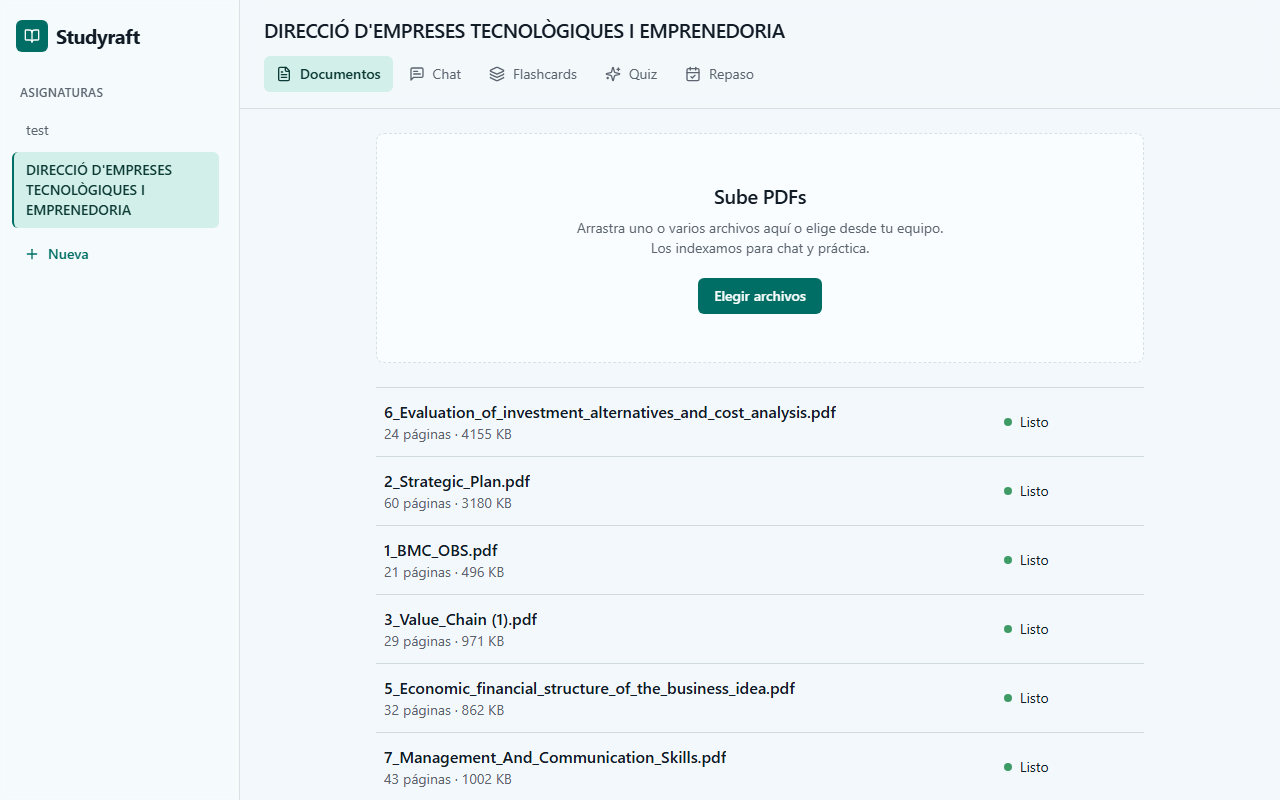
\includegraphics[width=0.92\textwidth]{figures/screenshots/04-documents.png}
\caption{Documents indexats en estat \emph{Listo} (RF-03). PDF de tema amb nom numerat (la llista es desplaça; el xat i el quiz en mostren vuit).}
\label{fig:ui-docs}
\end{figure}

\begin{figure}[htbp]
\centering
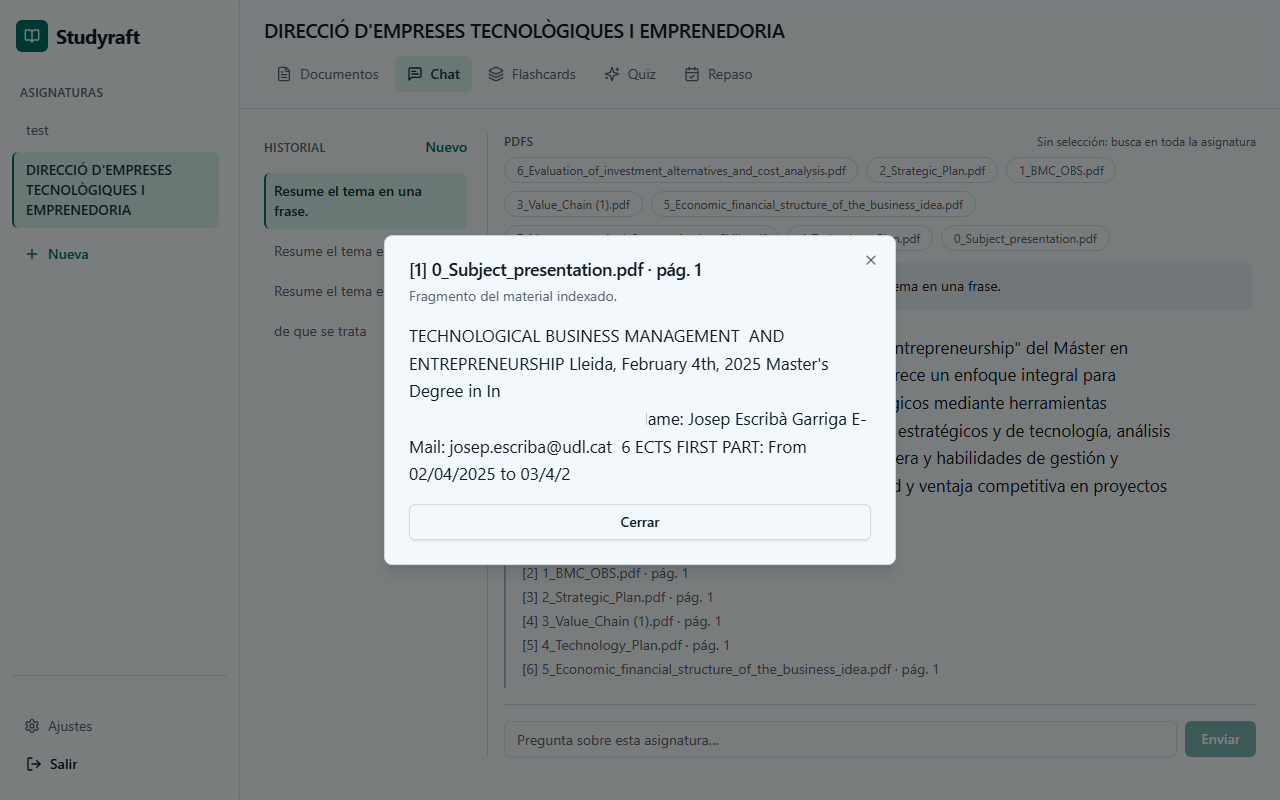
\includegraphics[width=0.92\textwidth]{figures/screenshots/05-chat.png}
\caption{Xat amb cita oberta: fitxer, pàgina i fragment indexat (RF-05 / RF-06). Correu de sessió i contacte del fragment, tapats.}
\label{fig:ui-chat}
\end{figure}

\paragraph{Recorregut de la figura~\ref{fig:ui-chat}.}
L'estudiant escriu «Resume el tema en una frase.»: intent \emph{resum} (capítol~\ref{sec:rag-pregunta}), sense filtre a un sol PDF. La resposta va en castellà de tu, ancorada al temari. La cita~\texttt{[1]} obre el fragment de \texttt{0\_Subject\_presentation.pdf}, pàgina~1 (presentació de l'assignatura). Això mostra el camí pregunta $\rightarrow$ intent $\rightarrow$ chunk citat; no mesura si cada oració de la resposta està al chunk.

\begin{figure}[htbp]
\centering
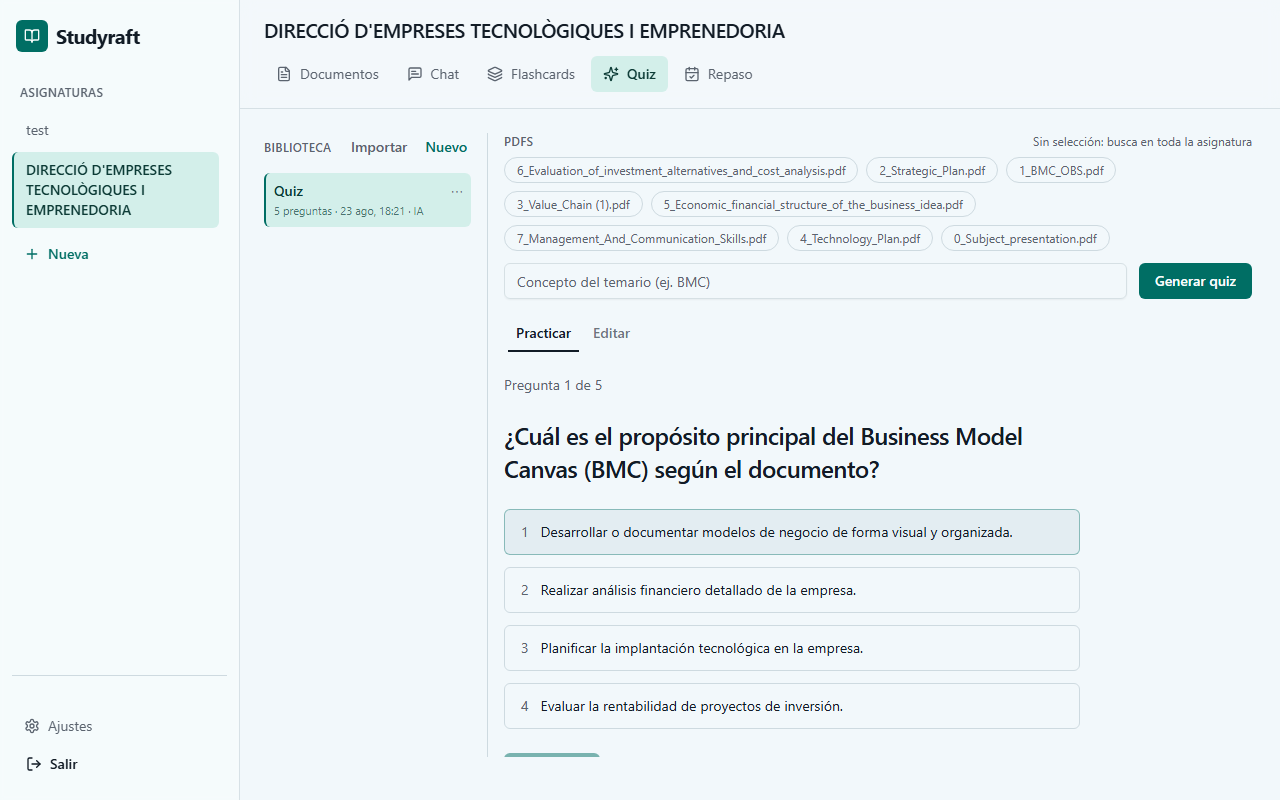
\includegraphics[width=0.92\textwidth]{figures/screenshots/06-quiz.png}
\caption{Qüestionari de pràctica generat sobre el corpus (RF-07): pregunta sobre el BMC, quatre opcions.}
\label{fig:ui-quiz}
\end{figure}

\begin{figure}[htbp]
\centering
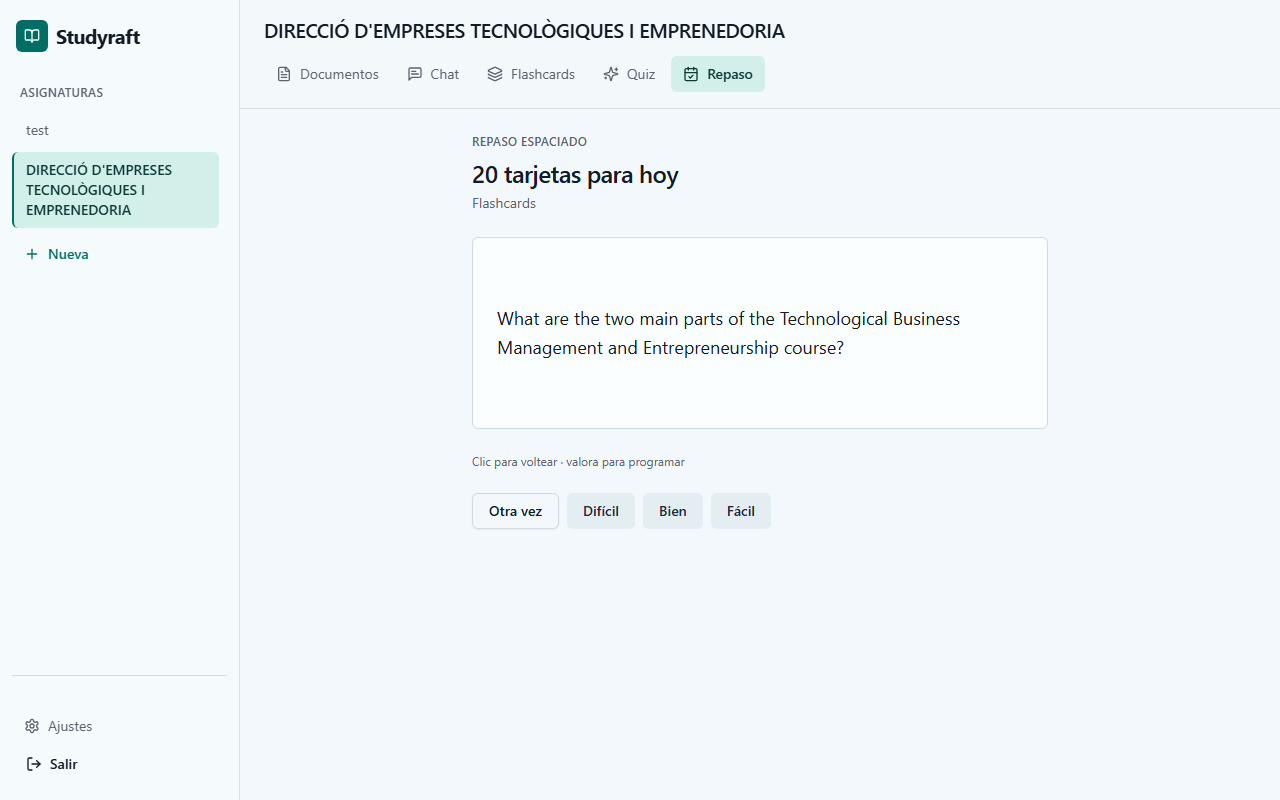
\includegraphics[width=0.92\textwidth]{figures/screenshots/08-planner.png}
\caption{Planner SM-2: targetes pendents d'avui i valoració de qualitat (RF-10).}
\label{fig:ui-planner}
\end{figure}

El qüestionari (figura~\ref{fig:ui-quiz}) es genera sobre el mateix índex; l'ítem visible pregunta el propòsit del BMC «según el documento». El planner (figura~\ref{fig:ui-planner}) mostra la cua del dia i els quatre botons SM-2 de la secció d'exemple numèric (capítol~\ref{cap:desarrollo}). Ni el quiz ni el planner tenen mètrica de qualitat pedagògica en aquest capítol.

\section{Amenaces a la validesa}

En experimentació, una \emph{amenaça a la validesa} és un motiu pel qual la mesura no vol dir el que sembla:

\begin{itemize}
  \item \textbf{Interna.} Un sol corpus i l'autor com a operador del CLI; no hi ha anotació cega de rellevància.
  \item \textbf{Externa.} Apunts d'una assignatura no representen tots els PDF (columnes, escanejos). El corpus és majoritàriament en anglès; les vuit consultes del CLI són en castellà i part de les cartes generades també surten en anglès: l'idioma no està controlat com a factor.
  \item \textbf{Constructe.} La latència de retrieval no és qualitat d'aprenentatge: un sistema ràpid pot citar el fragment equivocat. Les vuit consultes del CLI són factuals; no mesuren resum ni capítol.
  \item \textbf{Fiabilitat.} Les APIs d'LLM no són deterministes. El p50 d'híbrid depèn sobretot d'embeddings i Postgres; el del rerank, del LLM. La primera consulta infla el \texttt{max}.
\end{itemize}

\section{Limitacions observades al producte}

Cites amb snippet, no visor PDF. Agentic d'una sola reescriptura. El pipeline debug relança prerrequisits, no rehidrata artefactes intermedis persistits. La ingestió d'escanejos falla (esperat: PyPDF sense OCR). No s'ha cronometrat l'ingestió ni el xat extrem a extrem. Aquests límits es reprenen com a treball futur, no com a defectes ocults.

\chapter{Gestió, riscos, ètica i sostenibilitat}
\label{cap:gestion}

Aquest capítol recull tres qüestions sobre el sistema construït: en quin ordre s'ha muntat i per quina dependència; què pot fallar i quina decisió ja hi ha al repositori; qui paga què (hores acadèmiques, API de l'LLM, allotjament). El calendari, les 390\,h i els 9.750\,€ de dedicació són a la secció~\ref{sec:ambit-temporal}. Les alternatives de stack són a la taula~\ref{tab:decisiones}.

\section{Ordre d'enginyeria (després del prototip)}

El juliol de 2026 s'arxiva el llegat LangChain i es reescriu el producte actual. La taula~\ref{tab:ordre-eng} és la \textbf{dependència} entre peces, no un segon Gantt. Sense esquema i RLS no hi ha aïllament; sense ports no hi ha tests amb fakes; sense API no hi ha UI. La memòria va al final perquè documenta l'estat, no el pla inicial.

\begin{table}[htbp]
\centering
\caption{Ordre d'enginyeria del sistema actual i per què no es pot avançar el pas.}
\label{tab:ordre-eng}
\small
\begin{tabularx}{\textwidth}{c>{\raggedright\arraybackslash}p{3.4cm}X}
\toprule
Pas & Què es va fer & Dependència \\
\midrule
1 & Backend i frontend nets, \texttt{.env}, tooling & Sense això no hi ha projecte compilable. \\
2 & Migracions SQL 0001--0008 i RLS & El cas d'ús necessita \texttt{user\_id} i polítiques abans de pujar PDF. \\
3 & Domini, ports, adaptadors RAG i ingestió & El pipeline i el xat no poden parlar amb Postgres/OpenAI sense ports. \\
4 & API FastAPI (35 rutes) i JWT & La UI no crida el domini: crida HTTP autenticat. \\
5 & Next.js: auth SSR, assignatures, documents, xat, pràctica & Requereix l'API i les cookies de Supabase. \\
6 & Qualitat, Compose, flags (jeràrquic, agentic, rerank, planner) & Extras sobre un nucli ja testejable. \\
7 & Biblioteca d'artefactes (CRUD, pistes, import/export) & Requereix flashcards/quiz persistents, no només ``l'última generació''. \\
8 & Aquesta memòria \LaTeX{} & Documenta el que ja corre, no el que es preveia el desembre. \\
\bottomrule
\end{tabularx}
\end{table}

\section{Riscos del sistema construït}

Un \textbf{risc} és un esdeveniment que fa fallar l'objectiu (resposta inventada, quota esgotada, dades d'un usuari visibles a un altre). Mitigar no és ``ser-ne conscient'': és una decisió ja al codi. La taula~\ref{tab:riesgos} lliga cada risc a un residu honest: el que encara pot passar el dia de la defensa.

\begin{table}[htbp]
\centering
\caption{Riscos de Studyraft: on es veuen, què hi ha al repositori i què queda obert.}
\label{tab:riesgos}
\small
\begin{tabularx}{\textwidth}{>{\raggedright\arraybackslash}p{2.7cm}>{\raggedright\arraybackslash}p{5.0cm}X}
\toprule
Risc & Mitigació al repo & Residu \\
\midrule
L'LLM inventa fora dels apunts
  & RAG híbrid, cites \texttt{[n]}, prompt ``only the provided context'', política lecture-focused
  & No hi ha mètrica de fidelitat (capítol~\ref{cap:resultados}). \\
Quota o factura OpenAI
  & Defecte: rerank i agentic apagats; el proveïdor LLM es pot canviar a Gemini
  & Qualsevol pregunta encara gasta tokens (secció~\ref{sec:cost-api}). \\
Supabase pausa el projecte gratuït
  & Esquema al git (migracions); Compose no substitueix el Postgres allotjat
  & Sense projecte actiu no hi ha Auth ni Storage. \\
PDF escanejat (imatge)
  & Fora d'abast; el parse buit és un error visible a la UI
  & No hi ha OCR. \\
Llegat LangChain inmantenible
  & Reescriptura hexagonal; tests amb fakes, sense claus
  & El prototip resta arxivat, fora del camí de producció. \\
Abús de l'API (moltes preguntes)
  & Flags de límit (120 peticions/min) a la configuració
  & El middleware encara no aplica el límit (deute dit al capítol~\ref{cap:conclusiones}). \\
\bottomrule
\end{tabularx}
\end{table}

\section{Dades, privadesa i tercers}

Els PDF d'un estudiant poden contenir noms, correus o capítols de llibre. Studyraft no és un producte comercial, però \textbf{tracta dades}. La taula~\ref{tab:dades} diu què es queda al projecte Supabase i què surt cap a l'LLM. Això no és un dictamen legal.

\begin{table}[htbp]
\centering
\caption{Inventari de dades del MVP (un usuari, el seu projecte Supabase).}
\label{tab:dades}
\small
\begin{tabularx}{\textwidth}{>{\raggedright\arraybackslash}p{3.2cm}>{\raggedright\arraybackslash}p{3.4cm}X}
\toprule
Dada & On es guarda & Surts cap a OpenAI / Gemini? \\
\midrule
Compte (e-mail, JWT)
  & Supabase Auth
  & No. \\
PDF original
  & Storage (\texttt{documents})
  & No: l'API no reenvia el fitxer sencer. \\
Chunks i embeddings
  & Postgres (\texttt{pgvector})
  & Només els $k{=}8$ fragments del context d'una pregunta (i, si s'activa, candidats de rerank). \\
Fil de xat, cartes, ressenyes SM-2
  & Postgres, amb RLS
  & El text de la pregunta i la resposta generada, sí; l'historial SM-2, no. \\
\bottomrule
\end{tabularx}
\end{table}

Tres límits que el tribunal pot preguntar:

\begin{itemize}
  \item \textbf{Aïllament.} RLS amb \texttt{auth.uid()} al client i \texttt{user\_id} al cas d'ús amb service role (capítol~\ref{cap:arquitectura}). Un UUID endevinat no hauria de llistar documents d'altri; el service role \emph{sí} que pot, per això el backend ha de filtrar sempre.
  \item \textbf{Encàrrec a un tercer.} Els fragments recuperats viatgen al proveïdor LLM. No es pot prometre ``els apunts no surten mai del disc''. Cal dir-ho a la UI i aquí.
  \item \textbf{Ús legítim.} El TFM assumeix que qui puja el PDF en té dret. El corpus d'avaluació són apunts d'una assignatura cursada per l'autor; el PDF original no forma part del dipòsit. El sistema no s'ha d'usar per indexar material aliè.
\end{itemize}

Les captures del capítol~\ref{cap:resultados} tapen el correu de la sessió (peu de la barra) i, al fragment citat de la presentació de l'assignatura, el contacte del professor. El PDF de dipòsit no ha de servir com a llista d'adreces.

Si el centre exigeix un formulari oficial d'ètica (p.~ex.\ UPC), s'adjunta a part: aquesta secció no el substitueix. En termes de memòria (no és assessorament GDPR): la base és el consentiment de l'estudiant sobre els \emph{seus} apunts; la minimització (no cal retenir el PDF eternament) i l'esborrat (cascades SQL + Storage) són línies de producte, no tancades al MVP. El responsable del tractament, en un ús personal, és qui crea el projecte Supabase.

\section{Sostenibilitat (el que sí es pot afirmar)}

Cada ingestió crida el model d'embeddings un cop per chunk; el xat crida l'LLM; el rerank i l'agentic afegeixen crides. No es mesuren kWh del proveïdor: aquest TFM no té telemetria de datacenter. El que sí és una decisió de disseny és \textbf{no} encendre per defecte els bucles cars (taula~\ref{tab:flags-cost}). El Docker local no replica GPU: l'impacte energètic recau en OpenAI o Google.

\begin{table}[htbp]
\centering
\caption{Flags que multipliquen crides a GPU aliena. Defecte del producte (setembre 2026).}
\label{tab:flags-cost}
\small
\begin{tabularx}{\textwidth}{>{\raggedright\arraybackslash}p{3.6cm} l X}
\toprule
Paràmetre & Defecte & Efecte \\
\midrule
Proveïdor de rerank & \texttt{none} & Sense crida LLM extra per pregunta. \\
Agentic RAG & \texttt{false} & Sense reescriptura ni segona passada de retrieval. \\
RAG jeràrquic & \texttt{true} & Una crida d'LLM per sinopsi \emph{en ingestió} (un cop per document). \\
Proveïdor LLM & OpenAI & El port admet Gemini; els números d'aquesta secció són OpenAI. \\
\bottomrule
\end{tabularx}
\end{table}

\section{Cost: hores, allotjament i API}
\label{sec:cost-api}

Hi ha \textbf{tres comptes diferents}. Barrejar-los és el que fa incomprensible una sola taula de ``preus''.

\begin{enumerate}
  \item \textbf{Dedicació acadèmica.} 390\,h $\times$ 25\,€/h $=$ 9.750\,€ (secció~\ref{sec:ambit-temporal}). És el cost d'oportunitat del TFM, no una factura.
  \item \textbf{Allotjament.} El MVP usa un projecte Supabase del pla gratuït/pausable i Docker al portàtil. No hi ha tesi de negoci. En explotació caldria projecte de pagament, worker separat i retenció dels PDF.
  \item \textbf{API de models.} OpenAI cobra per \emph{token} (tros de text). Aquesta secció calcula \emph{només} aquest tercer compte, amb preus públics consultats l'1 de setembre de 2026 \parencite{openai-pricing}, sobre el corpus del capítol~\ref{cap:resultados}. \textbf{No és una factura del compte}: no s'han llegit consums reals.
\end{enumerate}

\subsection{Unitats i tarifes}

Un \textbf{token} és la unitat de facturació. Per a text en català/castellà, una regla grollera (la que usa OpenAI a la documentació) és $\approx 4$ caràcters per token. Studyraft no compta tokens exactes amb un tokenitzador a la ingestió: el càlcul d'aquí és un \textbf{sostre} (pitjor cas), perquè cada chunk té com a màxim 1200 caràcters.

Els models per defecte del repositori són l'\emph{embedding-3-small} (vector de 1536 dimensions) i \texttt{gpt-4.1-mini} (xat, rerank, generació de cartes). La taula~\ref{tab:tarifes} són preus per \textbf{un milió} de tokens. Per passar a dòlars d'una crida: $\mathrm{cost} = (\text{tokens}/10^{6})\times\text{preu}$. OpenAI factura en USD; no es converteix a euros per no fixar un tipus de canvi.

\begin{table}[htbp]
\centering
\caption{Tarifes públiques OpenAI usades en aquest capítol (1/09/2026). Font: pàgina d'API pricing.}
\label{tab:tarifes}
\small
\begin{tabularx}{\textwidth}{l X r}
\toprule
Model (defecte del repo) & Què factura & USD / 1M tokens \\
\midrule
Embeddings \emph{3-small} & Només entrada (el text del chunk) & 0,02 \\
\texttt{gpt-4.1-mini} & Entrada (prompt + context) & 0,40 \\
\texttt{gpt-4.1-mini} & Sortida (la resposta generada) & 1,60 \\
\bottomrule
\end{tabularx}
\end{table}

\subsection{Exemple A: indexar el corpus d'avaluació (una vegada)}

El capítol~\ref{cap:resultados} indexa una assignatura real amb \textbf{114 chunks}. Hipòtesi conservadora: cada chunk fa el màxim (1200 caràcters). El solapament de 150 caràcters duplica uns quants tokens; queda dins el mateix ordre de magnitud.

\begin{align*}
\text{tokens} &\approx 114 \times 1200 / 4 = 34\,200 \\
\text{cost embeddings} &= 34\,200 / 10^{6} \times 0{,}02\,\mathrm{USD} = 0{,}000684\,\mathrm{USD}
\end{align*}

És a dir: \textbf{menys d'un dècim de cèntim de dòlar} per deixar el temari cercable. Si el document té sinopsi jeràrquica activada, hi ha \emph{una} crida extra d'LLM per fitxer en ingestió, no 114: encara és cèntims, no euros. Reindexar cada dia sí que multiplicaria; el producte indexa en pujar el PDF, no en cada pregunta.

\subsection{Exemple B: una pregunta de xat (configuració per defecte)}

Per defecte no hi ha rerank ni agentic. El retrieval deixa $k{=}8$ chunks al prompt. Hipòtesi de sostre:

\begin{itemize}
  \item Context: $8 \times 1200$ caràcters $\approx 2400$ tokens, més rètols \texttt{[n]} / nom de fitxer ($\approx 150$).
  \item Prompt de sistema (``answer using only the provided context'') $\approx 100$ tokens.
  \item Pregunta de l'estudiant $\approx 50$ tokens.
  \item \textbf{Entrada total} $\approx 2700$ tokens.
  \item \textbf{Sortida} (resposta típica d'estudi) $\approx 300$ tokens.
\end{itemize}

\begin{align*}
\text{entrada} &= 2700 / 10^{6} \times 0{,}40 = 0{,}00108\,\mathrm{USD} \\
\text{sortida} &= 300 / 10^{6} \times 1{,}60 = 0{,}00048\,\mathrm{USD} \\
\text{una pregunta} &\approx 0{,}0016\,\mathrm{USD}
\end{align*}

Arrodonit a \textbf{0,002\,USD per pregunta} (dues dècimes de cèntim). Generar un conjunt de flashcards o un qüestionari és \emph{una altra} crida al mateix model, del mateix ordre: no és ``gratis'' respecte al xat, però tampoc és un altre esglaó de preu.

\subsection{Rerank LLM (opcional)}

Si s'activa el rerank amb LLM, abans del xat s'envien candidats (fins a 20, amb uns 500 caràcters cadascun) i el model retorna un JSON d'ordre. Això són $\approx 2500$ tokens d'entrada i $\approx 50$ de sortida $\approx 0{,}001\,\mathrm{USD}$ extra: la pregunta passa d'$\approx 0{,}002$ a $\approx 0{,}003\,\mathrm{USD}$. El p50 de latència del capítol~\ref{cap:resultados} puja $\approx 4\times$ (369\,ms $\rightarrow$ 1608\,ms) perquè s'espera la xarxa; el \emph{preu} no es multiplica per quatre, perquè la sortida del rerank és petita.

\subsection{Escenaris sobre aquest corpus}

La taula~\ref{tab:cost-escenaris} aplica els exemples A i B. ``Estudiant'' vol dir: corpus ja indexat, flags per defecte, sense reindexar.

\begin{table}[htbp]
\centering
\caption{Ordre de magnitud del cost d'API OpenAI sobre el corpus de 114 chunks. No és una factura.}
\label{tab:cost-escenaris}
\small
\begin{tabularx}{\textwidth}{X r r}
\toprule
Escenari (hipòtesis dels exemples A i B) & USD & Com es treu \\
\midrule
Indexar l'assignatura (1 vegada) & 0,0007 & Exemple A \\
1 pregunta de xat, sense rerank & 0,002 & Exemple B \\
10 preguntes / mes (un tema) & 0,02 & $10\times$ B \\
100 preguntes / mes (ús intensiu d'examen) & 0,16 & $100\times$ B \\
100 preguntes + rerank LLM a totes & 0,26 & $100\times(B+\text{rerank})$ \\
\bottomrule
\end{tabularx}
\end{table}

En conjunt, la dedicació del TFM són milers d'euros; el cost variable d'API d'un estudiant sobre \emph{aquesta} assignatura són \textbf{cèntims de dòlar al mes} si es deixen apagats agentic i rerank. El càlcul és un sostre amb tarifes públiques, no un preu garantit: canvia si OpenAI puja tarifes, si el chunk és més llarg, si el fil de xat reenvia tot l'historial, o si es reindexa el temari cada dia. El que el disseny controla és no encendre per defecte les crides extra (taula~\ref{tab:flags-cost}).

\chapter{Conclusions i treball futur}
\label{cap:conclusiones}

\section{Conclusions}

S'ha reconstruït un assistent d'estudi RAG amb un cicle complet ---ingerir PDF privats, recuperar fragments amb cites, generar i editar pràctica, programar el repàs SM-2--- sobre una arquitectura hexagonal, un backend FastAPI i un frontend Next.js, amb dades aïllades per RLS. El valor del treball és mostrar que un sistema d'IA aplicada es pot \emph{dissenyar} (capítol~\ref{cap:arquitectura}), \emph{implementar} amb límits visibles (capítol~\ref{cap:desarrollo}) i \emph{avaluar} amb protocol (capítol~\ref{cap:resultados}).

L'hexàgon ha permès tests sense claus d'LLM i canviar de proveïdor sense reescriure el xat. La recuperació híbrida combina senyal densa (paràfrasi) i lèxica (termes rars); RRF les fusiona sense un model extra. SM-2 al domini fa el calendari explicable (``aquesta carta surt avui perquè $q<3$'').

Respecte als objectius del capítol~\ref{cap:intro}:

\begin{itemize}
  \item O1--O5 estan \emph{implementats} en codi (API, UI, domini, biblioteca d'artefactes).
  \item O6 (avaluació) és \emph{parcial}: protocol, 63 tests unitaris, ruff/mypy nets, Vitest i Playwright smoke (taula~\ref{tab:calidad}), latència d'híbrid vs híbrid+rerank sobre 114 chunks (taula~\ref{tab:bench}), i un recorregut qualitatiu del cicle a la UI (secció~\ref{sec:cicle-ui}). No s'ha mesurat groundedness, ni una línia ``només dens'', ni ingestió, ni el xat extrem a extrem. La traçabilitat O1--O6 és a la taula~\ref{tab:trazas}.
\end{itemize}

El límit d'aquest treball és l'abast de l'avaluació: el sistema es prova com a programari i el retrieval té un p50 en un corpus. Això no substitueix un estudi d'aprenentatge, ni una prova que l'híbrid superi una línia només densa.

\section{Implantació real}

Per a un ús més enllà del TFM caldria: projecte Supabase en producció no pausat, secrets rotats, un worker d'ingestió separat del procés HTTP, implementació real del rate limit (el flag existeix; el middleware encara no), còpies de seguretat i pressupost d'embeddings. El Docker Compose de desenvolupament cobreix arrencar API i app, no un SLA.

\section{Línies futures}

\begin{enumerate}
  \item OCR / PDF escanejats (el parse buit avui és un error honest).
  \item Visor PDF sincronitzat amb la cita (pàgina + highlight), més enllà del snippet de 280 caràcters.
  \item Avaluació automàtica de fidelitat (groundedness) a més de latència.
  \item Cronometrar ingestió i el xat extrem a extrem; tres consultes d'intent (resum / capítol / factual) al mateix CLI.
  \item Agentic amb pressupost d'eines, no una sola reescriptura.
  \item FSRS o un altre model d'SRS si hi ha prou ressenyes per ajustar.
  \item Exportació Anki \texttt{.apkg} i moviment de cartes entre conjunts.
  \item Estudi d'usuaris ($n$ estudiants, qüestionari pre/post).
\end{enumerate}

Aquestes línies parteixen de límits de la tecnologia usada (extracció PyPDF, APIs tancades, anotació esbiaixada) i del que el capítol~\ref{cap:resultados} encara no mesura.


\printbibliography[heading=bibintoc,title={Bibliografia}]

\appendix
\chapter{Guia de desplegament i reproducció}
\label{anexo:despliegue}

Aquest annex resumeix com clonar i arrencar l'estat actual. El detall operatiu és al \texttt{README} de l'arrel del repositori.

\section{Repositori}

El codi font d'aquest TFM és a GitHub:

\begin{center}
\url{https://github.com/yanghao1005/rag-study-assistant}
\end{center}

\begin{lstlisting}
git clone https://github.com/yanghao1005/rag-study-assistant.git
\end{lstlisting}

El dipòsit a secretaria duu, a més, una còpia comprimida del projecte (sense secrets ni dependències instal·lades). El commit de referència és el de la data de lliurament.

\section{Serveis}

Desenvolupament local amb dos processos, o un sol Compose:

\begin{itemize}
  \item Backend al port 8000 (Uvicorn sobre \texttt{app.main:app}). El worker d'ingestió corre al mateix procés si la ingestió asíncrona és activa.
  \item Frontend: \texttt{pnpm dev} al directori de l'app (port 3000).
  \item Alternativa: \texttt{docker compose up --build} des de l'arrel (API 8000, app 3000).
\end{itemize}

\begin{lstlisting}
cd backend
PYTHONPATH=. python -m uvicorn app.main:app --reload --port 8000
\end{lstlisting}

\section{Migracions}

Aplicar les migracions \texttt{0001}--\texttt{0008} del directori SQL del backend al projecte Supabase (Auth + Storage + pgvector). La 0008 afegeix sinopsi de document i l'historial de ressenyes SM-2.

\section{Variables}

Copia els fitxers d'exemple d'entorn del backend i del frontend. No facis mai commit de secrets. Flags rellevants: RAG jeràrquic, RAG agentic, proveïdor de rerank i proveïdor LLM.

\section{Auth}

Habilita correu i, si s'usa, Google OAuth. Redirect de desenvolupament: \url{http://localhost:3000/auth/callback}.

\chapter{Esquema de dades i API}
\label{anexo:esquema}

\section{Taules de negoci}

Totes porten aïllament per usuari (RLS amb \texttt{auth.uid()} al client; \texttt{user\_id} al backend amb service role). Migracions \path{backend/supabase/migrations/} (0001--0008). El diagrama E-R simplificat és la figura~\ref{fig:er}.

\begin{description}
  \item[profiles] Preferències (nom, flag agentic). FK a \texttt{auth.users}.
  \item[subjects] Assignatura. FK usuari; esborrat en cascada cap a documents.
  \item[documents] PDF, estat d'ingestió, \texttt{synopsis} opcional. FK assignatura.
  \item[document\_chunks] Fragment: text, pàgines, embedding, FTS. FK document.
  \item[jobs, pipeline\_stage\_runs] Cua i traça d'etapes. FK document opcional.
  \item[fils i missatges de xat] Historial per assignatura.
  \item[study\_artifacts] Conjunt de flashcards o quiz (títol, origen, recència). FK assignatura.
  \item[flashcards, quiz\_questions] Ítems del conjunt. FK artefacte (cascada).
  \item[flashcard\_reviews] Historial SM-2. FK carta.
\end{description}

\section{Rutes HTTP (prefix \texttt{/api})}

Totes excepte salut requereixen JWT. Contracte Pydantic i OpenAPI: vegeu el paràgraf sota la taula.

\begin{table}[htbp]
\centering
\caption{Superfície HTTP (35 rutes en total; resum). El detall és a OpenAPI.}
\label{tab:api}
\small
\begin{tabularx}{\textwidth}{l>{\raggedright\arraybackslash\ttfamily}p{5.2cm}X}
\toprule
Mètode & Camí & Funció \\
\midrule
GET & /health & Salut (sense JWT) \\
GET/PATCH & /me & Perfil i flag agentic \\
GET/POST & /subjects & Llista / crea assignatura \\
GET/PATCH/DEL & /subjects/\{id\} & Detall assignatura \\
POST & /documents/upload & Pujada PDF + job \\
GET/DEL & /documents/\{id\} & Detall / esborra \\
POST & /documents/\{id\}/reindex & Relança ingestió \\
GET & /jobs/\{id\} & Estat del job \\
POST & /chat/ask, /chat/ask/stream & Xat JSON / SSE \\
POST & /generate/flashcards, /generate/quiz & Genera conjunt \\
CRUD & /generate/artifacts & Biblioteca \\
GET/POST & /planner/due, /planner/review & SM-2 \\
POST & /debug/pipeline & Debug (flag) \\
\bottomrule
\end{tabularx}
\end{table}

El detall de comportament (cues, SSE, SM-2) és als capítols~\ref{cap:arquitectura} i~\ref{cap:desarrollo}.
Les 35 rutes inclouen llista de documents, fragments per a cites, fils de xat i CRUD imbricat de cartes i preguntes; la taula n'és un extracte.
Els esquemes Pydantic viuen a \path{backend/app/entrypoints/api/schemas.py}; OpenAPI és \path{/api/docs} amb l'API en marxa.

\chapter{Protocol d'avaluació reproduïble}
\label{anexo:eval}

\section{Qualitat}

\begin{lstlisting}
cd backend
python -m pytest tests/unit -q
python -m ruff check app tests
python -m mypy app

cd ../frontend
pnpm exec tsc --noEmit
pnpm test
# pnpm build && pnpm test:e2e
\end{lstlisting}

\section{Benchmark de retrieval}

Requereix \texttt{.env} amb Supabase i embeddings, més un \texttt{user-id} i \texttt{subject-id} reals:

\begin{lstlisting}
cd backend
PYTHONPATH=. python -m app.entrypoints.cli.benchmark \
  --user-id <uid> --subject-id <sid> \
  --query "modelo de negocio" --query "propuesta de valor" \
  --query "lienzo canvas" --query "startup" \
  --query "innovacion" --query "financiacion" \
  --query "mercado objetivo" --query "equipo fundador"
\end{lstlisting}

El CLI sempre mesura cerca híbrida. El run publicat (taula~\ref{tab:bench}) va deixar $k=10$ chunks (defecte aleshores del port). El run amb rerank es fa amb el proveïdor LLM de rerank activat a l'\texttt{.env}. La sortida (p50, max, chunks) és la taula~\ref{tab:bench}.

\section{Integració real (opt-in)}

\begin{lstlisting}
# Windows PowerShell
$env:RUN_REAL_INTEGRATION="1"
python -m pytest tests/integration -v
\end{lstlisting}


\end{document}
